\documentclass[12pt]{article}
\usepackage[margin=1in]{geometry}
\usepackage{amsmath, amssymb, amsthm}
\usepackage{booktabs}
\usepackage{hyperref}
\usepackage{graphicx}
\usepackage{array}
\usepackage{xcolor}
\usepackage{titlesec}
\usepackage{abstract}
\usepackage{multirow}
\usepackage{float}
\usepackage{pgfplots}
\pgfplotsset{compat=1.18}
\usepackage{tikz}

\hypersetup{
    colorlinks=true,
    linkcolor=black,
    urlcolor=blue,
    citecolor=black
}

\newtheorem{theorem}{Theorem}
\newtheorem{definition}{Definition}
\newtheorem{proposition}{Proposition}

\title{\textbf{Beyond Accuracy: Toward a Fundamental Unit\\
of AI Cognitive Efficiency}}
\author{
    Winston Zai Lin \\
    \small Blair Academy \\
    \small \texttt{linzaiwinston413@gmail.com}
}
\date{March 2026}

\begin{document}
\maketitle

\begin{abstract}
Before a measurement unit can be adopted, three conditions must hold. It must be
\textbf{measurable}: computable from data anyone can access. It must be \textbf{stable}:
small errors in input should not flip the ranking. And it must be \textbf{reusable}: two
teams running the same protocol should get the same number, so results are comparable
across papers. Standard AI leaderboards satisfy none of these---they rank by benchmark
accuracy alone, with no compute adjustment, no stability guarantees, and no fixed protocol.

We introduce the \textbf{Cognitive Efficiency Score} (CES) as a framework proposal
designed to address all three conditions. CES divides bits of benchmark uncertainty
resolved by log-scaled inference FLOPs, normalized to a human expert baseline of 1.0. The
formula is computable from publicly available model cards, and its log-scaled denominator
is designed to compress FLOPs estimation noise. As an illustrative analysis, we apply CES
to 13 models using published benchmark scores and estimated FLOPs, finding that CES
rankings diverge substantially from accuracy rankings---Gemini Ultra ranks \#1 by MMLU
(90.4\%) but \#6 by CES due to its 1{,}000T FLOPs cost. We also propose the \textbf{Task
Efficiency Benchmark} (TEB), which measures the quantity CES approximates directly: human
time saved per task, adjusted for output quality. A feasibility pilot ($n=4$, 3 automated
tasks) yields $\rho(\mathrm{CES}, \mathrm{TEB}) = 0.80$ (95\% CI $[-0.10,\, 0.99]$;
establishes feasibility only). Full validation of CES against real deployment efficiency
at scale remains future work. Open-source implementation:
\url{https://github.com/WINSTON672/lin-score}.
\end{abstract}

%-----------------------------------------------------------
\section{Introduction}
%-----------------------------------------------------------

Three things kill a proposed measurement unit before anyone adopts it.

First, it is not \textbf{measurable}: the inputs require data nobody publishes, so the unit
exists in theory but cannot be computed in practice. Second, it is not \textbf{stable}:
small errors in the inputs---a 30\% FLOPs estimate error---flip the rankings, so the unit
cannot be trusted even when computed. Third, it is not \textbf{reusable}: different teams
make different choices about normalization, benchmark selection, and scale, so their numbers
cannot be compared across papers. A unit that fails any of these three conditions will not
be adopted.

There is no standard unit for AI cognitive efficiency, and this is why.

Every team deploying an LLM informally computes accuracy divided by cost and uses it to
make a selection decision. The problem is not that the idea is missing. The problem is
that without a fixed specification, every team does it differently---different benchmarks,
different cost estimates, different scales. The results are incomparable. And a specific
failure mode stays invisible: Gemini Ultra scores highest on raw accuracy (MMLU: 90.4\%)
and ranks \textit{sixth} by efficiency once compute is factored in, because its 1{,}000T
FLOPs costs $3\times$ more than the top compute-efficient model. Every standard leaderboard
misses this. It is not a corner case---it is the rule.

\textbf{This paper proposes a unit that satisfies all three conditions.} The
\textbf{Cognitive Efficiency Score} (CES) is bits of benchmark uncertainty resolved per
unit of log-scaled inference compute. The inputs are computable from any published model
card. The log-scaled denominator compresses FLOPs noise so that $\pm30\%$ estimation error
changes rankings by at most one adjacent swap ($\rho \geq 0.989$). The protocol is fully
specified---benchmark suite, weights, human anchor, normalization---so two independent teams
produce the same number for the same model.

Before the formula, Section~\ref{sec:conditions} establishes the three conditions formally
and shows why current metrics fail them. The formula in Section~\ref{sec:turing} follows
from those conditions. It is not a formula searching for a justification---it is the output
of asking: \textit{what is the simplest formula that is measurable, stable, and reusable
simultaneously?}

Shannon did not begin with $H = -\sum p \log p$ and then explain why it was useful. He
began with a definition---one bit resolves a single binary uncertainty---and showed the
formula followed from it. The same logic applies here. The definition comes first: cognitive
efficiency is bits of uncertainty resolved per unit of computational work. The formula is
what you get when you apply that definition to measurable quantities under the three
conditions.

\textbf{Contributions.} (1)~Three conditions for a legitimate AI efficiency unit
(Section~\ref{sec:conditions}). (2)~CES---the Turing unit definition and measurement
pipeline satisfying all three (Sections~\ref{sec:turing}--\ref{sec:results}). (3)~TEB---the
first formalization of direct deployment efficiency measurement, with a feasibility pilot
yielding $\rho(\mathrm{CES}, \mathrm{TEB}) = 0.80$ (Section~\ref{sec:teb}).

%-----------------------------------------------------------
\section{Related Work}
%-----------------------------------------------------------

\subsection{Compute Efficiency}

Hoffmann et al.\ \cite{hoffmann2022} (Chinchilla) showed models are undertrained relative to parameter count. Kaplan et al.\ \cite{kaplan2020} established log-linear scaling laws between compute and capability. Neither produces a deployable inference efficiency unit.

\subsection{Benchmark Aggregation}

HELM \cite{liang2022} and the Open LLM Leaderboard aggregate benchmarks into composite scores. Chatbot Arena \cite{chiang2024} uses human preference Elo ratings. All measure capability in isolation, divorced from compute cost.

\subsection{Most Closely Related: Intelligence per Watt}

Saad-Falcon et al.\ \cite{saadfalcon2024} measured task accuracy per watt of hardware power across 20+ models, finding 5.3$\times$ IPW improvement from 2023--2025. CES differs in three ways: (1)~\textbf{hardware independence} --- CES uses FLOPs (intrinsic to the model), not watts (hardware-dependent); (2)~\textbf{information-inspired proxy} --- CES uses Shannon entropy reduction as an approximation of resolved uncertainty, not raw accuracy; (3)~\textbf{standardized relative scale} --- CES is anchored to 1.0 = human expert, enabling interpretable protocol-consistent comparisons (unlike watts, which have no natural intelligence anchor).

\subsection{AI Cognitive Impact}

Kosmyna et al.\ \cite{kosmyna2025} found LLM-assisted writers showed weaker neural coupling and poorer recall than unaided writers, coining the term ``cognitive debt'' for the accumulated cognitive cost of AI dependency. Macnamara et al.\ \cite{macnamara2024} showed AI assistance accelerates skill decay without performers' awareness. No prior work quantifies cognitive impact with a standard unit paired to an efficiency measure.


%-----------------------------------------------------------
\section{Three Conditions for a Legitimate Measurement Unit}
\label{sec:conditions}
%-----------------------------------------------------------

A measurement unit is legitimate when researchers who disagree about everything else can
still agree to use it---because it is computable, stable, and produces the same number
across independent teams. We formalize this as three conditions. CES is then derived in
Section~\ref{sec:turing} as the formula that satisfies all three.

\subsection{Condition 1: Measurability}

A unit is measurable if its inputs are publicly available and the computation requires no
proprietary data or privileged access.

\textbf{What this requires for an AI efficiency unit.} Capability must be estimable from
published benchmark scores. Compute must be estimable from published model cards or
standard architecture formulae. A measure requiring internal model weights, token-level
log-probabilities from closed models, or privately held FLOPs measurements is not
measurable in this sense---only the model developer can compute it.

\textbf{Why existing metrics fail.} Intelligence-per-watt~\cite{saadfalcon2024} requires
physical access to deployment hardware. Exact entropy computation requires per-question
log-probabilities, which no major closed model provider publishes. Raw accuracy / raw FLOPs
is computable, but because FLOPs are only estimated for closed models, no prior work
specifies whether rankings survive that estimation uncertainty---measurability requires not
just computability but documented robustness.

\textbf{How CES addresses this condition.} CES requires (1)~aggregate benchmark accuracy
$b_i$, published in every model card; and (2)~estimated inference FLOPs $C(M)$, derivable
from parameter counts for open models and architecture disclosures for closed models. The
computation is a six-step pipeline executable in under an hour from published data.
Experiment~4 (Section~\ref{sec:exp4-pilot}) demonstrates end-to-end computability: starting
from zero, querying models via public API, scoring responses, and computing CES takes under
10 minutes. What this does not demonstrate is that the resulting number captures efficiency
for any specific deployment---benchmark accuracy is a population-level proxy, not a
task-specific measurement. Closing that gap is the purpose of TEB (Section~\ref{sec:teb}).

\subsection{Condition 2: Stability}

A unit is stable if small errors in its inputs produce small errors in its outputs---rankings
do not flip when inputs change by a plausible estimation error.

\textbf{What this requires.} For an AI efficiency unit, the dominant error source is FLOPs
estimation: proprietary models do not publish exact inference FLOPs, so practitioners
estimate from parameter counts and published architecture details. Independent estimates can
vary by $\pm30\%$ for the same model. Stability under this error is therefore the relevant
test: do rankings hold when all FLOPs estimates are perturbed by $\pm30\%$?

\textbf{Why this is a non-trivial constraint.} A linear denominator ($I/C$) is highly
sensitive near ranking boundaries---a 30\% shift in $C$ changes the denominator by 30\%,
and models at similar efficiency levels swap ranks. This is why raw accuracy/FLOPs is
insufficient as a unit: the compute sensitivity makes it unstable.

\textbf{How CES addresses stability.} The log-scaled denominator $\log_2(1+C)$ is the
critical design choice. Because $\log$ is compressive, a 30\% error in $C$ translates to
a much smaller error in $\log_2(1+C)$. For a model with $C=600$T FLOPs, a $\times1.3$
perturbation changes the denominator from $\log_2(601) \approx 9.23$ to $\log_2(781)
\approx 9.61$---a $4.1\%$ shift, not 30\%. Section~\ref{sec:exp2} shows that under
$\pm30\%$ uniform FLOPs perturbation across the 13-model illustrative dataset, $\rho \geq
0.989$ with only one adjacent-rank swap. This is a sensitivity analysis on estimated
data---it demonstrates the log-scaling property, but is not an independent empirical
validation of stability under real-world deployment conditions.

\subsection{Condition 3: Reusability}

A unit is reusable if two independent teams computing it on the same model get the same
number. This requires a complete protocol specification: not just a formula, but a fixed
benchmark suite, fixed weights, a fixed human reference anchor, and a fixed normalization
convention.

\textbf{Why this is the hardest condition.} Measurability is achieved by choosing computable
inputs. Stability follows from a design choice (log-scaling). Reusability requires
specifying every implementation decision so that no choice is left to the researcher. Every
ad hoc variation---which benchmarks, what weights, whose brain-compute estimate---produces a
number that cannot be compared with others computed under different choices. The informal
accuracy-over-compute ratio practitioners already use informally fails this condition
entirely: 13 teams doing it informally produce 13 incomparable numbers.

\textbf{How CES addresses reusability.} Four choices are fixed by protocol: (1)~benchmark
suite (MMLU + HumanEval, with exact versions and evaluation configuration);
(2)~benchmark weights (variance-optimal: $w_M = 0.47$, $w_{HE} = 0.53$, derivation in
Section~\ref{sec:pipeline}); (3)~human expert anchor ($\mathcal{T}(\mathcal{H}) \approx
0.0718$ raw Turing at Moderate tier); (4)~normalization convention (raw Turing divided by
human reference). Two teams following the same protocol produce the same number for the
same model. What is not yet established is whether that number transfers across deployment
contexts---whether a CES computed on MMLU+HumanEval predicts efficiency on a different
task distribution. Protocol reusability (same benchmark $\Rightarrow$ same number) is
satisfied by specification; deployment reusability requires empirical validation at scale.

\subsection{CES as the Solution}

Given these three conditions, the formula is not a free choice---it falls out.

Measurability constrains the inputs: aggregate benchmark accuracy and estimated FLOPs.
Stability constrains the denominator: it must be log-scaled to compress compute noise.
Reusability constrains the protocol: every design decision must be fixed and published.
Combine all three and you get:
\begin{equation}
\mathcal{T}(M) = \frac{I(M)}{\log_2(1 + C(M))} \quad [\text{Turing}]
\end{equation}
where $I(M)$ is weighted bits of benchmark uncertainty resolved and $C(M)$ is estimated
inference FLOPs. This is the \textbf{Turing}---a unit of cognitive efficiency. The
\textbf{Cognitive Efficiency Score} (CES) is the standardized protocol for computing it
from public data. The next section derives both formally and shows exactly what each term
measures.

%-----------------------------------------------------------
\section{The Turing: A Unit of Cognitive Efficiency}
\label{sec:turing}
%-----------------------------------------------------------

\subsection{Definition From First Principles}

Before deriving the formula, we define the quantity the formula measures. The unit that falls out of this definition --- bits of uncertainty resolved per unit of log-scaled inference compute --- we call the \textbf{Turing} ($\mathcal{T}$), after Alan Turing, whose foundational work on computation and machine intelligence makes him the natural namesake for a unit measuring how efficiently a system does cognitive work. The tradition of naming units after their field's founders --- Hertz, Watt, Pascal, Shannon --- is one this unit follows. The \textbf{Cognitive Efficiency Score} (CES) is the standardized measurement protocol for computing a model's value in Turing from publicly available benchmark data.

\textbf{What is cognitive work?} A cognitive task presents a system with uncertainty: multiple possible answers, with one correct. Resolving that uncertainty constitutes cognitive work. The natural measure is Shannon entropy reduction---the difference between the uncertainty before and after the system responds.

Given a task with $k$ equally plausible options, prior uncertainty is $H_0 = \log_2 k$ bits. A system that answers correctly with probability $p$ induces posterior entropy:
\begin{equation}
H_{\text{post}}(p, k) = -p\log_2 p - (1-p)\log_2\frac{1-p}{k-1}
\end{equation}

The cognitive work performed is the uncertainty resolved:
\begin{equation}
\Delta H(p, k) = H_0 - H_{\text{post}}(p, k) = \log_2 k + p\log_2 p + (1-p)\log_2\frac{1-p}{k-1}
\end{equation}

This is zero at random chance ($p = 1/k$), one bit at perfect binary accuracy ($k=2$, $p=1$), and monotonically increasing for $p > 1/k$. Cognitive work is not proportional to accuracy---it is proportional to \textit{uncertainty resolved}.

\textbf{What is computational work?} A system expends computational work to produce a response. The natural measure is floating-point operations (FLOPs) during inference---hardware-independent and intrinsic to the model. However, empirical scaling laws \cite{kaplan2020, hoffmann2022} establish that model capability grows approximately as the \textit{logarithm} of compute: doubling FLOPs produces sublinear capability gains. The effective computational work in cognitive terms therefore scales as $\log_2 C$, not $C$. We define it as $\log_2(1 + C)$, where the $+1$ prevents singularity at $C = 1$ TFLOP.

\textbf{Cognitive efficiency defined.} Cognitive efficiency is the ratio of cognitive work performed to computational work expended:
\begin{equation}
\mathcal{T}(M) = \frac{\mathbb{E}[\Delta H(p, k)]}{\log_2(1 + C(M))} \quad [\mathrm{Turing}]
\end{equation}

where the expectation is over a standardized distribution of tasks. \textit{This definition precedes the formula.} The formula is what you get when you apply this definition to measurable quantities. CES is not constructed to produce a number; the number follows from the definition.

\textbf{From definition to measurement.} In practice, $\mathbb{E}[\Delta H]$ is estimated from a benchmark suite: a finite set of tasks with known correct answers, weighted by domain coverage and discriminative power. The weighted estimate is $I(M) = \sum_i w_i \alpha_i \cdot \Delta H(b_i, k_i)$, where $b_i$ is empirical accuracy on benchmark $i$. CES is the empirical instantiation of cognitive efficiency on a specific benchmark suite---not an ad-hoc ratio, but a measurement procedure derived from the definition above.

\subsection{The Measurement Gap}

The definition above is exact. The measurement is not. Understanding what is lost in the transition from definition to measurement is essential to using CES correctly.

\textbf{What the definition requires.} Computing $\Delta H(p, k)$ exactly requires knowing the model's true probability $p$ of answering correctly on a given question---its full posterior distribution over $k$ options. This is available only for open-weight models where token-level log-probabilities can be extracted. For closed models (GPT-4, Claude, Gemini), it is not published.

\textbf{What the measurement uses instead.} In place of $p$, CES substitutes aggregate benchmark accuracy $b_i$: the fraction of questions answered correctly across the test set. This introduces two approximation steps.

\textit{Step 1: Per-question probability replaced by aggregate accuracy.} Aggregate accuracy $b_i$ is the mean of per-question outcomes $\{0, 1\}$. Using it as a proxy for $p$ conflates two things: a model that answers every question with $p = 0.82$ (calibrated, uniform) and a model that answers 82\% of questions with $p = 1.0$ and 18\% with $p = 0.0$ (deterministic, overconfident). Both yield $b_i = 0.82$ but resolve different amounts of uncertainty. Because bits\_resolved is convex, Jensen's inequality guarantees that the per-question average entropy reduction $\frac{1}{n}\sum_i \Delta H(p_i, k)$ is always at least as large as $\Delta H(\bar{b}, k)$. CES therefore \textit{underestimates} true cognitive work. The bias magnitude is approximately $\frac{1}{2} f''(\bar{b}) \sigma_b^2$ where $f''(b) = 1/(b(1-b)\ln 2)$; for a typical model with $\bar{b} = 0.82$ and $\sigma_b \approx 0.15$, the underestimation is roughly $0.11$ bits per question, or $\sim$35\% of the total resolved.

\textit{Step 2: Correctness used as proxy for genuine uncertainty reduction.} Even with exact per-question probabilities, $\Delta H(p, k)$ measures how much uncertainty an observer has about the \textit{benchmark answer}---not how much the model understands the underlying domain. A model that has memorized the benchmark answers and a model that genuinely reasons to the correct answer are indistinguishable in $\Delta H$ if their accuracy distributions match. This is not a flaw in the definition; it is a limitation of what benchmarks can measure. Benchmarks test whether the correct answer is produced, not whether the reasoning behind it is sound.

\textbf{What this means for interpretation.} CES measures \textit{benchmark-proxy cognitive efficiency}: the efficiency of the approximation to cognitive work that benchmarks afford, not cognitive work in its full theoretical sense. This is not a failure of the metric---it is an honest account of what is observable. The definition establishes the target. The measurement is the best available proxy for that target given publicly accessible data. The gap between them is the research agenda: better access to model internals, per-question log-probabilities, and richer task formats would each close a different part of the gap.

\textbf{When the gap matters.} The gap is small when models are well-calibrated ($\sigma_b$ is low, per-question accuracy is near-uniform) and large when models are inconsistent (high $\sigma_b$, some questions always right and others always wrong). For frontier models on standard benchmarks, calibration tends to be moderate; for specialized or fine-tuned models with uneven competence, the aggregate approximation is less reliable. CES$_{\text{pq}}$ (per-question variant, defined in Section~\ref{sec:pipeline}) eliminates Step 1 when per-question labels are available and is the recommended form for open-weight model evaluation.

\noindent\textbf{Notation summary.}
\begin{center}
\small
\begin{tabular}{ll}
\toprule
\textbf{Symbol / Acronym} & \textbf{Meaning} \\
\midrule
Turing, $\mathcal{T}$ & Unit of cognitive efficiency (bits per log-FLOP) \\
CES & Cognitive Efficiency Score: the protocol for measuring $\mathcal{T}(M)$ \\
$\mathcal{T}(M)$ & Turing value of model $M$ (raw: bits/log-FLOP; normalized: relative to human expert) \\
$I(M)$ & Weighted information score (bits resolved per query) \\
$C(M)$ & Estimated inference FLOPs (teraFLOPs, log-scaled) \\
$b_i$, $k_i$ & Accuracy and answer-choice count on benchmark $i$ \\
$w_i$, $\alpha_i$ & Benchmark weight; discriminative weight \\
$K_{85}$, $R_{85}$ & Human expert reference values on MMLU and HumanEval \\
$\rho$ & Spearman rank correlation \\
\bottomrule
\end{tabular}
\end{center}

\subsection{Information-Theoretic Foundation}

Shannon entropy of a discrete random variable $X$:
\begin{equation}
H(X) = -\sum_x P(x)\log_2 P(x)
\end{equation}

For a $k$-choice question, a model answering correctly with probability $p$ resolves:
\begin{equation}
\text{bits\_resolved}(p) = 1 + p\log_2 p + (1-p)\log_2(1-p)   \quad (k=2)
\end{equation}
\begin{equation}
\text{bits\_resolved}(p,k) = \log_2 k + p\log_2 p + (1-p)\log_2\!\left(\frac{1-p}{k-1}\right)   \quad (k>2)
\end{equation}

Key properties: at $p=0.5$ (random guessing) the value is $0$; at $p=1.0$
(perfect accuracy) the value is $1$; monotonically increasing for $p > 0.5$;
convex (bits\_resolved$' = \log_2(p/(1-p))$ is increasing), so marginal gains \textit{increase} as accuracy approaches~1 --- each additional percentage point near $p=1$ resolves more bits than the same gain near $p=0.5$. \textbf{Design note:} this convex reward is appropriate when near-perfect accuracy matters (e.g., safety-critical deployment), but may over-weight marginal gains in contexts where moderate accuracy suffices. Section~\ref{sec:compute-norm} shows that replacing the log-scaling denominator with $\sqrt{C}$ or $C^{0.25}$ yields similar rankings ($\rho \geq 0.87$), indicating robustness; practitioners requiring saturating numerator behavior should consider the saturation-corrected form in Section~\ref{sec:failure-cases}.

\noindent\textbf{Aggregate accuracy approximation.} In practice, $p$ is computed as the aggregate accuracy across $n$ benchmark questions, not as a per-question probability. This introduces a systematic approximation: bits\_resolved$(p) = 1 - H(p)$ where $H(p)$ is the strictly \textit{concave} binary entropy, so bits\_resolved is strictly \textit{convex} for $p \in (0,1)$. Jensen's inequality for convex functions therefore gives $\text{bits\_resolved}(\bar{p}) \leq \mathbb{E}[\text{bits\_resolved}(p_i)]$. I therefore \textit{underestimate} true information resolution relative to the per-question ideal: the aggregate approximation yields a lower information score than the per-question average, making the metric conservative. The correct quantity is $\frac{1}{n}\sum_{i=1}^n \text{bits\_resolved}(p_i)$, which requires per-question pass/fail labels (available for open benchmarks) or per-question log-probabilities (available only for open-weight models). Where per-question data is available, the per-question average is preferred and labeled CES$_{\text{pq}}$. \textbf{Bias magnitude.} By the second-order Taylor expansion, the gap is approximately $\frac{1}{2} f''(\bar{p})\,\sigma_p^2$ where $f''(p) = 1/(p(1-p)\ln 2)$. For a typical model with $\bar{p} = 0.82$ and per-question standard deviation $\sigma_p \approx 0.15$, the underestimation gap is $\approx \tfrac{1}{2} \cdot (0.82 \times 0.18 \times 0.693)^{-1} \cdot 0.023 \approx 0.11$ bits, roughly $35\%$ of bits\_resolved$(0.82) \approx 0.31$. The aggregate approximation additionally underestimates the advantage of high-variance models: a model with heterogeneous per-question performance (higher $\sigma_p$) has strictly higher true information than a uniform model at the same $\bar{p}$, but the aggregate approximation assigns them identical scores.

\subsection{Formal Definition}

\begin{definition}[The Turing]
The \textbf{Turing} is the unit of cognitive efficiency. One Turing is the cognitive efficiency of a system that resolves one bit of benchmark uncertainty per unit of log-scaled inference compute:
\begin{equation}
1\ \mathrm{Turing} \equiv \frac{1\ \mathrm{bit}}{\log_2(1\ \mathrm{TFLOP}\ \text{increment})}
\end{equation}
The Turing value of model $M$ is:
\begin{equation}
\boxed{\mathcal{T}(M) = \frac{I(M)}{\log_2(1 + C(M))} \quad [\mathrm{Turing}]}
\end{equation}
where $I(M)$ is the weighted bits resolved across benchmarks (the cognitive work), and $C(M)$ is total inference FLOPs normalized to 1 TFLOP (the computational work). This is a raw value in Turing. For interpretability, scores are reported normalized to the human expert reference: $\mathcal{T}_{\mathrm{norm}}(M) = \mathcal{T}(M) / \mathcal{T}(\mathcal{H})$, where $\mathcal{T}(\mathcal{H}) \approx 0.0718\ \mathrm{Turing}$ is the human expert's raw value. The normalized scale sets human expert performance to 1.0 --- a reference point, not a definition of the unit.
\end{definition}

\begin{definition}[Cognitive Efficiency Score (CES)]
The \textbf{Cognitive Efficiency Score} is the standardized protocol for measuring a model's Turing value from publicly available benchmark data. CES specifies: (1)~the benchmark suite and weights, (2)~the compute estimation procedure, (3)~the human expert reference values, and (4)~the normalization convention. Two models' CES values are directly comparable only when computed under identical protocol versions. For standard (non-reasoning) models, $C(M)$ is the single-pass forward-pass FLOPs. For chain-of-thought reasoning models (o1, o3, DeepSeek-R1), $C(M) = C_R + C_O$ where $C_R$ is reasoning FLOPs and $C_O$ is output-generation FLOPs; the decomposed variants $\mathcal{T}_R = I(M)/\log_2(1+C_R)$ and $\mathcal{T}_O = I(M)/\log_2(1+C_O)$ are defined in Section~\ref{sec:decomposed-ces}.
\end{definition}

\noindent\textbf{Epistemic status.} CES is an \textit{accuracy-over-compute heuristic}, not a measure of general intelligence or true information transfer. The \textit{bits resolved} numerator applies a monotonic nonlinear transformation to benchmark accuracy that shares the mathematical form of Shannon entropy reduction but does not measure genuine cognitive work: it quantifies how much uncertainty an observer has about the correct answer to a benchmark question, not how much the model understands the domain. A model that memorizes answers and a model that genuinely understands the domain are indistinguishable in CES if their aggregate accuracies match. Accuracy is treated as a \emph{proxy} for uncertainty reduction, not as a direct measurement of it. Three limitations follow directly: (i)~a model that has memorized benchmark answers scores identically to one that genuinely understands the domain; (ii)~bits resolved on different task types are not intrinsically comparable without calibrated $\alpha_i$; (iii)~CES is meaningful only when comparing models evaluated on identical benchmark configurations. Researchers should report CES alongside domain-stratified subscores and calibration metrics (Section~\ref{sec:calibrated-ces}) to avoid overinterpreting the aggregate. \textbf{Alternative proxy}: negative log-likelihood (NLL) per question is more sensitive to calibration than accuracy: $\text{bits\_NLL}(M,i) = -\frac{1}{|B_i|}\sum_{q \in B_i} \log_2 P_M(\text{correct} \mid q)$. NLL-based CES rewards confident correct answers and penalizes uncertain ones; it subsumes CES\_cal for models that publish token-level probabilities. Where log-probabilities are unavailable (most closed models), accuracy-based CES with the ECE penalty (CES\_cal) is the recommended approximation.

\noindent\textbf{Stabilization.} The $+1$ in the denominator ensures it is strictly positive for all $C(M) > 0$, removing the singularity at $C(M) = 1$ TFLOP (where $\log_2(1) = 0$). For all models in this paper, $C \gg 1$, so $\log_2(1+C) \approx \log_2 C$ to within 0.01\%.

\noindent\textbf{Dimensionlessness.} $I(M)$ is a weighted average of entropy differences (dimensionless). $C(M)$ is a pure number. $\mathcal{T}(M)$ is a ratio of two dimensionless quantities.

\noindent\textbf{Index, not universal unit.} CES is a \textit{normalized index}, not an invariant physical unit. Unlike the bit (Shannon) or the Hertz, CES scores depend on three measurement-protocol choices: (1)~the benchmark suite, (2)~the benchmark weights, and (3)~the human reference anchor. These are analogous to choosing a base year and coverage definition for a price index like CPI. Two CES scores are directly comparable only when computed under an identical protocol. Published CES scores must state the benchmark suite version, weights, and brain-compute tier. This does not diminish interpretability --- GDP is also a context-sensitive index, yet it is the field's most useful economic measure.

\noindent\textbf{Bounds.} $\mathcal{T}(M) \geq 0$ for all models with $p \geq 0.5$ on all benchmarks. There is no finite theoretical ceiling; the Human Expert Reference (1.0 CES) serves as the practical upper anchor.

\noindent\textbf{What $C(M)$ is not.} $C(M)$ is inference FLOPs --- not token count. Token count measures output length; FLOPs measure computational work regardless of verbosity. CES uses FLOPs as a \textit{proxy for thinking cost}, not a direct measurement. FLOPs do not capture memory access patterns, hardware utilization efficiency, MoE routing overhead, or sparsity effects (all addressed in Assumption~3 and Section~\ref{sec:decomposed-ces}). The denominator is more precisely described as ``log-scaled estimated computational work'' rather than ``thinking cost.''

\subsection{Information Score}

\begin{equation}
I(M) = \sum_{i} w_i \cdot \alpha_i \cdot \text{bits\_resolved}(b_i, k_i)
\end{equation}

where $\alpha_i$ is the \textbf{task complexity coefficient} for benchmark $i$, empirically estimated to correct for the fact that equal bits resolved on different task types does not imply equal cognitive difficulty. Without $\alpha_i$, a 1-bit gain on a 4-choice MMLU question would be treated as identical to a 1-bit gain on a binary code-pass test, despite the latter requiring substantially more generative reasoning. In the baseline implementation, $\alpha_{\text{MMLU}} = 1.0$ and $\alpha_{\text{HumanEval}} = 1.0$ (i.e., no correction).

\noindent\textbf{Variance-based calibration (recommended).} Benchmarks are not equally discriminative. A principled $\alpha_i$ uses the cross-model information variance:
\begin{equation}
\alpha_i = \frac{\sigma_i}{\bar{\sigma}}, \quad
\sigma_i = \mathrm{Std}_{M}\bigl[\mathrm{bits\_resolved}(b_i^{(M)}, k_i)\bigr]
\end{equation}
where $\sigma_i$ is the standard deviation of bits\_resolved across models on benchmark $i$ and $\bar{\sigma}$ is the mean. A benchmark where all models cluster near 90\% receives low $\alpha_i$. On my 13-model sample (computing $\sigma_i$ from bits\_resolved values, consistent with the formula): $\sigma_{\text{MMLU}} = 0.166$, $\sigma_{\text{HumanEval}} = 0.184$, yielding $\alpha_{\text{MMLU}} = 0.95$, $\alpha_{\text{HumanEval}} = 1.05$ before renormalization --- nearly equal, confirming that MMLU and HumanEval contribute comparable discriminative signal after entropy conversion. Baseline $\alpha_i = 1.0$ is retained for comparability with existing leaderboards.

\textbf{Sample-dependence caveat.} The variance-based weights $w_i \propto \sigma_i$ are computed from the same 13-model evaluation sample, creating a mild circularity: the weights depend on the observed model distribution and may not generalize to a model set with different capability spread. A model distribution heavy in sub-50\% HumanEval models would reduce $\sigma_{\text{HE}}$ and shift weight toward MMLU. The principled remedy is to pre-register weights from a held-out reference set or from domain-coverage rationale. The baseline (0.60, 0.40) weights use the latter approach and are sample-independent. The $\rho = 0.994$ agreement between baseline and variance-optimal rankings confirms the practical impact is small for this sample.

Baseline implementation uses two benchmarks. Weights were set to reflect general vs.\ code deployment balance and to maximize total discriminative variance across models:
\begin{equation}
w_i^* = \frac{\sigma_i}{\sum_j \sigma_j}, \quad \sigma_i = \mathrm{Std}_{M}\bigl[\mathrm{bits\_resolved}(b_i^{(M)}, k_i)\bigr]
\end{equation}
On my 13-model sample, computing $\sigma_i$ from bits\_resolved values (consistent with the formula): $\sigma_{\text{MMLU}} = 0.166$, $\sigma_{\text{HumanEval}} = 0.184$, giving variance-optimal weights $w_{\text{MMLU}}^* = 0.474$, $w_{\text{HumanEval}}^* = 0.526$. The baseline (0.60, 0.40) slightly up-weights MMLU to reflect its broader domain coverage (57 subjects vs.\ code only). The Spearman rank correlation between CES rankings computed under baseline (0.60, 0.40) and variance-optimal (0.47, 0.53) weights is $\rho = 0.994$ across all 13 models, confirming that the choice is practically inconsequential. Both choices are defensible; the sensitivity analysis in Section~5 shows rankings are stable under weight perturbation.

\noindent\textbf{Benchmark covariance and interaction effects.} The linear aggregation $I(M) = \sum_i w_i I_i$ implicitly assumes benchmark scores are independent. In practice, benchmarks share latent abilities: MMLU math questions and GSM8K both require arithmetic reasoning, so including both would partially double-count mathematical ability. Variance-optimal weights mitigate this by down-weighting low-variance benchmarks, but do not eliminate shared information. A principled correction is to replace scalar weights with a precision-weighted (covariance-adjusted) combination:
\begin{equation}
I_{\mathrm{cov}}(M) = \mathbf{w}^\top \mathbf{b}(M), \quad \mathbf{w} \propto \boldsymbol{\Sigma}^{-1}\mathbf{1}
\end{equation}
where $\boldsymbol{\Sigma}$ is the $n \times n$ cross-model covariance matrix of bits\_resolved values and $\mathbf{1}$ is the ones vector. This is the minimum-variance linear combination and penalizes redundant benchmarks. For the two-benchmark baseline (MMLU, HumanEval), Experiment~1 shows the CES--MMLU Spearman rank correlation is $\rho = 0.725$, indicating partial but not full redundancy between the benchmarks in the suite. The covariance-adjusted and variance-optimal rankings are Spearman $\rho \approx 0.99$ for the current two-benchmark suite; adding a third correlated benchmark (e.g., GSM8K) would widen the gap. Covariance adjustment is recommended when the benchmark suite exceeds three tasks with known overlap.

\begin{table}[H]
\centering
\begin{tabular}{lccl}
\toprule
\textbf{Benchmark} & $k$ & \textbf{Weight} & \textbf{Measures} \\
\midrule
MMLU \cite{hendrycks2021} & 4 & 0.47 & 57-domain knowledge and reasoning \\
HumanEval \cite{chen2021} & 2 & 0.53 & Code generation, functional correctness \\
\bottomrule
\end{tabular}
\caption{Baseline benchmark suite. Weights sum to 1.}
\end{table}

\subsection{Geometric Mean Alternative}
\label{sec:geometric-mean}

The baseline linear aggregation allows strong performance on one benchmark to compensate for failure on another. For deployments where \textit{zero competence in any domain is disqualifying} (e.g., a coding assistant must code), a geometric mean alternative enforces strict domain requirements:
\begin{equation}
I_{\mathrm{geom}}(M) = \prod_{i} \bigl[\text{bits\_resolved}(b_i, k_i)\bigr]^{w_i}
\end{equation}
Under geometric aggregation, $\text{bits\_resolved}(b_i) = 0$ on \textit{any} benchmark forces $I_{\mathrm{geom}} = 0$ regardless of performance elsewhere. This is strictly stronger than the linear floor: under the baseline, a model with zero HumanEval score can still earn $I = w_{\text{MMLU}} \cdot \text{bits}_{\text{MMLU}} > 0$; under geometric aggregation, it scores $I_{\text{geom}} = 0$ identically.

On my 13-model sample, models with $b_{\text{HE}} \leq 0.5$ already have $\text{bits\_resolved} = 0$ on HumanEval (both forms agree for these models). For the remaining 10 models, the Spearman rank correlation between linear and geometric CES is $\rho = 0.97$, indicating that aggregation choice is practically inconsequential for competent models. The linear baseline is retained throughout this paper for comparability with existing leaderboards; geometric aggregation is recommended for single-domain deployment decisions (e.g., selecting a code generation assistant, where any coding failure is unacceptable). \textbf{Minimum-performance gate.} To prevent strategic benchmark specialization under linear aggregation, a hard minimum gate can be enforced: CES is reported as $\mathcal{T} = 0$ for any model where $b_i < 0.5$ on any benchmark in the suite, regardless of other scores. This is already implicit in the bits\_resolved formula (sub-random accuracy gives zero bits), but can be made explicit as a reporting standard: a model that fails to exceed chance on any evaluated capability should not receive a positive CES score. This gate is equivalent to the geometric form's zero-collapse for the specific threshold $b_i = 0.5$.

\subsection{Domain-Stratified CES Scores}

For deployment decisions, the aggregate CES decomposes by task type:
\begin{align}
\mathcal{T}_{\text{knowledge}}(M) &= \frac{\text{bits\_resolved}(b_{\text{MMLU}})}{\log_2(1+C(M))} \\
\mathcal{T}_{\text{code}}(M)      &= \frac{\text{bits\_resolved}(b_{\text{HumanEval}})}{\log_2(1+C(M))} \\
\mathcal{T}_{\text{reasoning}}(M) &= \frac{\text{bits\_resolved}(b_{\text{GSM8K}})}{\log_2(1+C(M))}
\end{align}

Aggregate $\mathcal{T}$ is the weighted mean. A model with high $\mathcal{T}_{\text{code}}$ but low $\mathcal{T}_{\text{knowledge}}$ is the right tool for a coding assistant, not a research assistant --- even at similar aggregate CES. \textbf{Cross-domain validity caveat}: $\mathcal{T}_{\text{knowledge}}$ and $\mathcal{T}_{\text{code}}$ are validated on MMLU and HumanEval respectively; they should not be extrapolated to domains not covered by those benchmarks (e.g.\ $\mathcal{T}_{\text{reasoning}}$ requires GSM8K or equivalent). Any new domain requires its own benchmark with a stated $\alpha_i$ and $k_i$.

\subsection{Assumptions}

\begin{enumerate}
    \item \textbf{Benchmark accuracy serves as an information-inspired efficiency proxy.} CES inherits the strengths and weaknesses of the underlying benchmarks. Accuracy is not equated with intelligence; it is treated as a proxy for entropy reduction.
    \item \textbf{Domain scope.} CES validity is restricted to domains covered by the benchmark suite. The baseline (MMLU + HumanEval) covers natural language understanding and code generation. CES computed on this suite should \emph{not} be interpreted as a measure of multimodal, mathematical reasoning, scientific discovery, or creative generation capability. Cross-domain validity requires benchmark suites validated for each target domain.
    \item \textbf{Inference FLOPs are the relevant cost.} Training cost, memory bandwidth, and energy are not captured. FLOPs are treated as architecture-independent: a MoE model routing to 2 of 8 experts and a dense model with identical active-parameter FLOPs are assigned the same $C(M)$. In practice, MoE routing introduces memory-access overhead that FLOPs do not capture, and hardware kernel efficiency varies by architecture. Published CES scores should note whether FLOPs were measured (via profiling) or estimated from parameter counts; estimated MoE FLOPs carry additional uncertainty beyond the $\pm30\%$ baseline.
    \item \textbf{Training compute is excluded.} CES measures deployment-time efficiency. A full lifecycle cost would amortize training compute over the model's query lifetime: $C_{\text{total}} = C_{\text{train}} / N_{\text{queries}} + C_{\text{inference}}$. At large scale ($N \sim 10^{12}$ queries), the amortized term is negligible; at small deployment scale, training cost dominates. CES as defined is appropriate for comparing deployed models at scale; full lifecycle CES is a natural extension for model procurement decisions.
    \item \textbf{Correctness is binary.} Partial credit is not modeled. The $k$-choice formula assumes uniform wrong-answer distribution; future work should model confusion matrices.
    \item \textbf{Human expert is the appropriate anchor.} I normalize to 85th-percentile domain expert performance.
    \item \textbf{Log-scaling is the chosen compute transformation, with a principled justification.} Kaplan et al.\ \cite{kaplan2020} establish that model capability scales as a power law with training compute: $L \propto C^{-\alpha}$. Taking logarithms, capability is approximately linear in $\log C$ --- equal log-compute increments buy roughly equal capability steps. Adopting $\log_2 C$ as the cost denominator therefore measures efficiency per compute-doubling, the natural unit given the scaling laws regime. \textbf{The $+1$ regularization} in $\log_2(1+C)$ is not ad hoc: it is the standard $\log(1+x)$ transform for non-negative rate data \cite{shannon1948}, which (a)~prevents a singularity at $C=0$, (b)~recovers approximately linear cost for small $C$ (since $\log_2(1+C) \approx C/\ln 2$ for $C \ll 1$), and (c)~recovers $\log_2 C$ for large $C$ where the power-law regime holds. The transition between the two regimes occurs around $C \approx 1$T FLOPs, safely below all models evaluated. Section~\ref{sec:compute-norm} evaluates four alternative normalization functions and confirms rankings are robust ($\rho \geq 0.87$).
\end{enumerate}

\subsection{The Human Expert Reference Standard}

In the baseline configuration, CES is normalized so that \textbf{human expert performance $= 1.0$ CES}. This anchor is one of several normalization choices (see multi-anchor alternative below and Section~\ref{sec:compute-norm}):
\begin{equation}
\mathcal{T}(M) = \frac{\text{raw}(M)}{\text{raw}(\mathcal{H})} = \frac{I(M)/\log_2(1+C(M))}{I(\mathcal{H})/\log_2(1+C(\mathcal{H}))}
\end{equation}

Human reference values (baseline):
\begin{itemize}
    \item MMLU: $K_{85} = 0.898$ (Hendrycks et al.\ \cite{hendrycks2021} report human expert performance at the 85th percentile across evaluated domains; I use this directly as the MMLU anchor)
    \item HumanEval: $R_{85} = 1.0$ (Chen et al.\ \cite{chen2021} note that competent professional engineers solve $\approx 100\%$ of HumanEval problems given unlimited time; I use this as the ceiling anchor for code)
    \item Brain compute: $C(\mathcal{H}) = 1{,}000$T (Moravec \cite{moravec1998} moderate tier)
    \item Resulting: $\text{raw}(\mathcal{H}) = 0.715 / \log_2(1001) \approx 0.715 / 9.967 \approx 0.0718$
\end{itemize}

\noindent\textbf{Anchor uncertainty.} The 85th-percentile anchor is a point estimate, not a distribution. Human expert performance varies by domain, age, fatigue, and test format; the ``85th percentile'' is itself estimated from a finite sample of human test-takers. A more honest treatment represents the anchor as an interval: $K_{85} \in [0.87, 0.92]$ (plausible range from Hendrycks et al.\ variance across domains). This propagates to a CES uncertainty band of approximately $\pm 3\%$ on top models, narrower than the FLOPs uncertainty band ($\pm 5$--$8\%$). Since anchor uncertainty and FLOPs uncertainty are independent, the combined uncertainty is $[\mathcal{T}^-, \mathcal{T}^+]$ as reported in Table~\ref{tab:ces-extended}, which already accounts for the dominant source (FLOPs). Benchmark accuracy uncertainty (finite test-set sampling variance) adds a further $\pm 1$--$2\%$ for standard benchmark sizes ($n \geq 1{,}000$ questions). All three uncertainty sources are smaller than the rank gaps between adjacent CES models (median gap $\approx 0.06$), confirming that the reported rankings are robust to measurement error.

Sensitivity to the brain compute tier is significant. Table~\ref{tab:tier-sensitivity} shows CES scores under three Moravec tiers for representative models.

\begin{table}[H]
\centering
\small
\begin{tabular}{lcccc}
\toprule
\textbf{Model} & \textbf{Raw} & \textbf{Conserv.\ (10T)} & \textbf{Moderate (1000T)} & \textbf{High ($10^{16}$T)} \\
\midrule
GPT-4o        & 0.0559 & 0.249 & 0.718 & 3.827 \\
Llama-3-70B   & 0.0509 & 0.227 & 0.653 & 3.487 \\
GPT-4         & 0.0402 & 0.179 & 0.516 & 2.755 \\
GPT-3.5-Turbo & 0.0075 & 0.033 & 0.096 & 0.512 \\
\bottomrule
\end{tabular}
\caption{CES under three brain-compute tiers (variance-optimal weights $w_M=0.47, w_{HE}=0.53$). Rankings are tier-invariant ($\rho = 1.0$), while absolute values scale with $\log_2(1+C_H)$. At the High tier ($10^{16}$T), CES exceeds 1.0 because the extreme human-reference compute makes the human anchor less efficient than the AI models relative to that anchor --- mathematically consistent but physically implausible. The Moderate tier (1,000T) is the recommended default. Published CES must state the tier used.}
\label{tab:tier-sensitivity}
\end{table}

All scores in this paper use the Moderate tier. Rankings are \textit{tier-invariant}: the Spearman rank correlation across tiers is $\rho = 1.0$ for all 13 models, confirming that the normalization choice affects scale but not ordering.

\noindent\textbf{Combined uncertainty across all sources.} Three independent error sources contribute to CES point estimates: (1)~FLOPs estimation ($\pm 30\%$, dominant for proprietary models, characterized in Experiment~2); (2)~benchmark accuracy sampling error ($\pm 1$--$2\%$ for $n \geq 1{,}000$ questions, propagates to $\pm 1$--$2\%$ on CES); and (3)~anchor uncertainty ($K_{85} \in [0.87, 0.92]$, propagates to $\pm 3\%$ on CES). Treating the three sources as independent, the combined interval width is $\sqrt{(6\text{--}8\%)^2 + (2\%)^2 + (3\%)^2} \approx 7$--$9\%$ of the reported CES value. This combined interval is smaller than the median rank gap between adjacent models in Table~\ref{tab:ces-main} (median $\approx 0.060$, or $\sim 8\%$ of the top model's score), meaning adjacent-rank pairs near this gap threshold should be interpreted cautiously. The extended CES table (Table~\ref{tab:ces-extended}) reports the FLOPs-only CI $[\mathcal{T}^-, \mathcal{T}^+]$, which represents the dominant uncertainty source; full propagation would widen these intervals by roughly $1.3\times$. A Monte Carlo propagation jointly sampling FLOPs, accuracy, and anchor uncertainty is feasible where per-question data are available and is recommended for high-stakes deployment comparisons.

\textbf{Multi-anchor normalization (robust alternative).} To reduce dependence on a single contested constant, CES can be normalized against a \textit{reference set} rather than a single point:
\begin{equation}
\mathcal{T}_{\text{multi}}(M) = \frac{\text{raw}(M)}{\mu_{\text{ref}}}, \quad
\mu_{\text{ref}} = \frac{1}{|\mathcal{R}|}\sum_{r \in \mathcal{R}} \text{raw}(r)
\end{equation}
where $\mathcal{R}$ is a reference set containing at minimum: (1) human expert ($C = 1{,}000$T), (2) human average ($C = 1{,}000$T, lower accuracy), and (3) a small-model baseline (e.g.\ GPT-3.5-Turbo). This transforms CES into a stable relative scale insensitive to any single anchor. Results in this paper use single-anchor (human expert) normalization for simplicity; multi-anchor normalization is recommended when anchoring uncertainty is a concern. For reference, computing $\mu_\text{ref}$ as the mean of (human expert, human average at 65th pct., GPT-3.5-Turbo) yields a Spearman $\rho = 1.00$ with the single-anchor ranking across all 13 models --- confirming that the anchor choice affects scale but not ordering. See also the sensitivity analysis in Section~\ref{sec:compute-norm}.

\subsection{Worked Example}
\label{sec:worked-example}

For GPT-4o (MMLU $= 88.7\%$, HumanEval $= 90.2\%$, FLOPs $= 600$T), using \textbf{baseline weights} ($w_M=0.60$, $w_{HE}=0.40$). Under variance-optimal weights ($w_M=0.47$, $w_{HE}=0.53$), the result is $\mathcal{T} \approx 0.718$ as reported in Table~\ref{tab:ces-main}:
\begin{align}
\text{bits\_resolved}(0.887) &\approx 0.491 \\
\text{bits\_resolved}(0.902) &\approx 0.537 \\
I(\text{GPT-4o}) &= 0.60 \times 0.491 + 0.40 \times 0.537 \approx 0.510 \\
\log_2(1 + 600) &\approx 9.231 \\
\mathcal{T}(\text{GPT-4o}) &= (0.510/9.231)/(0.715/9.967) \approx 0.770
\end{align}

\subsection{Standardized Computation Pipeline}
\label{sec:pipeline}

For audit and benchmark reproducibility, CES scores must be computed via the following fixed pipeline:

\begin{enumerate}
    \item \textbf{Raw accuracy}: obtain $b_i \in [0,1]$ for each benchmark $i$ under standardized evaluation (zero-shot unless otherwise noted)
    \item \textbf{Convert to bits}: compute $\text{bits\_resolved}(b_i, k_i)$ using the $k$-choice formula
    \item \textbf{Apply task coefficients}: multiply by $\alpha_i$ (default $\alpha_i = 1.0$)
    \item \textbf{Apply weights}: compute $I(M) = \sum_i w_i \cdot \alpha_i \cdot \text{bits\_resolved}(b_i, k_i)$
    \item \textbf{Compute denominator}: $\log_2(1 + C(M))$ using reported or measured inference FLOPs
    \item \textbf{Normalize}: divide by $\text{raw}(\mathcal{H})$ using the stated brain-compute tier
\end{enumerate}

Published CES scores must report: benchmark versions, FLOPs source, brain compute tier, $\alpha_i$ values, contamination status, decoding temperature, and prompt format.

\noindent\textbf{Reproducibility note for Experiment~4.} All queries used greedy decoding (temperature $= 0$, top-$p = 1.0$). MCQ prompts: \texttt{"Question: [text]\textbackslash nOptions: A)~... B)~...\textbackslash nAnswer:"}; response extracted by first matching letter A--D. Code prompts: \texttt{"Write a Python function.\textbackslash n[docstring]\textbackslash nSignature: [sig]"}; response extracted as the first fenced code block. Full templates and test harness are in \texttt{verify\_experiments.py} at the repository.

\subsection{Decomposed CES for Reasoning Models}
\label{sec:decomposed-ces}

For chain-of-thought models (o1, o3, DeepSeek-R1), thinking tokens constitute the majority of inference FLOPs but are invisible in the output. Reporting total FLOPs $C = C_R + C_O$ underestimates the efficiency gap between reasoning and non-reasoning models. Two decomposed variants are defined:
\begin{equation}
\mathcal{T}_R(M) = \frac{I(M)}{\log_2(1+C_R)}, \qquad
\mathcal{T}_O(M) = \frac{I(M)}{\log_2(1+C_O)}
\end{equation}
$\mathcal{T}_R$ measures reasoning efficiency (quality per thinking cost); $\mathcal{T}_O$ measures output efficiency (quality per generation cost). For non-reasoning models, $C_R = 0$ and $\mathcal{T} = \mathcal{T}_O$. Published CES for o-series models must state which variant is reported and the $C_R / C_O$ split.

\subsection{Agentic CES}
\label{sec:agentic-ces}

Tool-using agents (with access to search, code interpreters, calculators) invoke external compute not counted in $C(M)$. The \textbf{Agentic CES} includes total-system compute:
\begin{equation}
\mathcal{T}_{\text{agent}}(M, \mathbf{T}) = \frac{I(M)}{\log_2\!\left(1 + C(M) + \sum_{j} n_j \cdot C_{T_j}\right)}
\end{equation}
where $n_j$ is the number of calls to tool $T_j$ and $C_{T_j}$ is its per-call FLOPs. Agentic CES is always $\leq \mathcal{T}(M)$; the gap quantifies the compute overhead of tool use. Systems with high $\mathcal{T}(M)$ but low $\mathcal{T}_{\text{agent}}$ are efficient models coupled to expensive tools. Representative per-call FLOPs estimates for common tools (order-of-magnitude; use measured values where available):
\begin{center}\small
\begin{tabular}{lll}
\toprule
\textbf{Tool} & $C_{T_j}$ \textbf{(TFLOP/call)} & \textbf{Source} \\
\midrule
Web search (index lookup) & $\approx 0.1$ & Network I/O dominated \\
Code execution (Python, 1s) & $\approx 0.01$ & CPU FLOP estimate \\
Calculator (arithmetic)     & $\approx 10^{-6}$ & Negligible \\
Image generation (SDXL)     & $\approx 5$--$20$ & GPU inference \\
LLM sub-call (GPT-4o level) & $\approx 600$ & Same as model FLOPs \\
\bottomrule
\end{tabular}
\end{center}

\subsection{Calibrated CES}
\label{sec:calibrated-ces}

CES rewards correctness but ignores confidence calibration. A model that answers correctly with 99\% confidence scores identically to one that answers correctly with 51\% confidence. The \textbf{calibrated CES} penalizes miscalibration:
\begin{equation}
\mathcal{T}_{\text{cal}}(M) = \mathcal{T}(M) \cdot \bigl(1 - \mathrm{ECE}(M)\bigr)
\end{equation}
where $\mathrm{ECE}(M) \in [0,1]$ is the Expected Calibration Error \cite{guo2017}. A perfectly calibrated model has $\mathrm{ECE} = 0$ and $\mathcal{T}_{\text{cal}} = \mathcal{T}$. A highly miscalibrated model ($\mathrm{ECE} = 0.3$) receives a 30\% penalty. Calibrated CES is recommended for safety-critical deployments.

%-----------------------------------------------------------
\section{Illustrative Analysis}
\label{sec:results}
%-----------------------------------------------------------

\noindent\textit{Note: The following analysis applies the CES formula to 13 models using
benchmark accuracy values and FLOPs estimates drawn from published model cards and
technical reports. This is not an original experiment---it is an illustration of what the
framework produces when applied to publicly available data. The purpose is to show that
CES rankings differ from accuracy rankings in practically meaningful ways, not to validate
CES as an empirically established unit.}

\bigskip

\subsection{Three Illustrative Calculations}
\label{sec:illustrative}

Before presenting the full 13-model results, three concrete calculations demonstrate that each metric produces new information not available from existing benchmarks. These use only publicly reported numbers; full sources are in Table~\ref{tab:data-sources}.

\medskip
\noindent\textbf{Calculation 1 (CES) --- benchmark rank $\neq$ efficiency rank.}
GPT-4 (MMLU $= 86.4\%$, FLOPs $= 1{,}800$T) outranks Llama-3-70B (MMLU $= 82.0\%$, FLOPs $= 70$T) on every standard accuracy leaderboard. Applying the six-step pipeline (Section~\ref{sec:pipeline}) with variance-optimal weights ($w_M=0.47$, $w_{HE}=0.53$):

\begin{center}
\small
\begin{tabular}{lcccc}
\toprule
\textbf{Step} & \textbf{Formula} & \textbf{GPT-4} & \textbf{Llama-3-70B} & \textbf{Source}\\
\midrule
Accuracy      & $b_M$, $b_{HE}$    & 86.4\%, 87.0\%       & 82.0\%, 80.5\% & Table~\ref{tab:data-sources} \\
Bits resolved & $1+p\log_2 p+(1-p)\log_2(1-p)$ & 0.426,\ 0.442 & 0.320,\ 0.290 & Eq.~(2) \\
Info score    & $I = 0.47b_M + 0.53b_{HE}$ & $0.434$       & $0.304$        & Eq.~(5) \\
Log compute   & $\log_2(1+C)$      & $10.81$              & $6.15$         & Table~\ref{tab:data-sources} \\
Raw CES       & $I/\log_2(1+C)$    & $0.0401$             & $0.0495$       & Def.~1 \\
\textbf{CES}  & raw / raw$({\mathcal{H}})$ & $\mathbf{0.517}$ & $\mathbf{0.633}$ & Def.~1 \\
\bottomrule
\end{tabular}
\end{center}

GPT-4's raw efficiency is $0.0401$; Llama-3-70B's is $0.0495$ --- a $23\%$ higher raw score driven by its $26\times$ compute advantage. Normalizing to the human expert anchor does not change the ordering. MMLU alone predicts GPT-4 wins; CES reveals Llama-3-70B wins. This ranking difference ($\Delta\text{CES} = 0.116$) is larger than the median adjacent-rank gap (0.06), confirming the divergence is not noise.

\bigskip

\noindent\textbf{Model selection.} The thirteen models were selected by two criteria: (1)~publicly reported MMLU and HumanEval scores are available in the literature as of the evaluation date, and (2)~estimated inference FLOPs are available from published model cards or independent profiling. All models satisfying both criteria that span at least four model families (GPT, Claude, Gemini, Llama/open-source), three compute tiers (small: $<10$T; medium: $10$--$200$T; large: $>200$T), and three generation cohorts (2022--2026) were included. This is a \textit{data-availability-constrained purposive sample}, not a random draw from the population of deployed LLMs. Spearman correlations on this 13-model sample characterize the framework's behavior on these specific models; population-level extrapolation requires a randomly drawn, pre-registered evaluation set.

\subsection{Data Sources and Reproducibility}
\label{sec:data-sources}

Table~\ref{tab:data-sources} lists the exact source document for each model's MMLU accuracy, HumanEval accuracy, and FLOPs estimate. Any third party can reproduce Table~\ref{tab:ces-main} by retrieving the accuracy values from the cited sources, applying the six-step pipeline in Section~\ref{sec:pipeline}, and using the FLOPs values below.

\noindent\textbf{FLOPs estimation method.} For open-weight dense models, FLOPs are computed via the standard transformer formula: $C \approx 2 \times N_{\text{params}} \times L$, where $N_{\text{params}}$ is non-embedding parameter count and $L = 512$ tokens (zero-shot default). For mixture-of-experts models (Mixtral-8x7B), $N_{\text{params}}$ is the \textit{active} parameter count (2 of 8 experts per token $\times 7$B = 13.5B active, rounded to 14B, $C \approx 46.7$T). For proprietary models (GPT-4, GPT-4o, Claude-3 family, Gemini), FLOPs are model-card estimates based on published architecture disclosures and carry $\pm 30\%$ uncertainty; this is the uncertainty characterized in Experiment~2.

\noindent\textbf{Choice count ($k$) clarification and known inconsistency.} MMLU is a 4-choice test ($k=4$), but for all models evaluated here (closed and open), only aggregate pass rates are publicly available --- per-choice token probabilities are not reported by providers. The baseline implementation therefore uses $k=2$ (binary correct/incorrect, Eq.~2) for all benchmarks, treating each question as a Bernoulli trial. This matches the worked example (Section~\ref{sec:worked-example}) and all CES values in this paper. \textbf{Limitation}: using $k=2$ discards the original entropy structure of MMLU ($k=4$ spans $\log_2 4 = 2$ maximum bits vs.\ $k=2$'s 1-bit ceiling), making absolute bits-resolved values incomparable across benchmarks with different $k$ when all are collapsed to $k=2$. The impact on rankings is mitigated by the consistent application of $k=2$ to all models: ordinal comparisons within a $k=2$ evaluation are valid. For open-weight models where per-choice log-probabilities are available, the $k=4$ formula (Eq.~3) is recommended and produces substantially higher bits-resolved values (e.g., GPT-3.5-Turbo MMLU: $k=4$ gives $\approx 1.14$ bits vs.\ $k=2$ gives $\approx 0.30$ bits at 70.0\%); any published CES score using $k>2$ must state this explicitly and must not be compared directly with $k=2$ scores.

\begin{table}[H]
\centering
\small
\begin{tabular}{lp{4.2cm}p{2.4cm}r}
\toprule
\textbf{Model} & \textbf{Accuracy Source} & \textbf{FLOPs Basis} & \textbf{FLOPs (T)} \\
\midrule
GPT-4o         & OpenAI GPT-4o System Card \cite{openai2024gpt4o}           & Model card est. & 600 \\
Llama-3-70B    & Meta Llama 3 Technical Report \cite{meta2024llama3}         & Param.\ formula & 70 \\
Claude-3-Opus  & Anthropic Claude 3 Model Card \cite{anthropic2024claude3}   & Model card est. & 500 \\
Claude-3-Haiku & Anthropic Claude 3 Model Card \cite{anthropic2024claude3}   & Model card est. & 20 \\
GPT-4          & OpenAI GPT-4 Technical Report \cite{openai2023gpt4}         & Model card est. & 1{,}800 \\
Gemini Ultra   & Gemini Technical Report \cite{google2023gemini}             & Model card est. & 1{,}000 \\
Claude-3-Sonnet & Anthropic Claude 3 Model Card \cite{anthropic2024claude3}  & Model card est. & 200 \\
Phi-3-mini     & Phi-3 Technical Report \cite{microsoft2024phi3}             & Param.\ formula & 3.8 \\
Llama-3-8B     & Meta Llama 3 Technical Report \cite{meta2024llama3}         & Param.\ formula & 8 \\
Gemini Pro     & Gemini Technical Report \cite{google2023gemini}             & Model card est. & 340 \\
Mixtral-8x7B   & Mixtral Technical Report \cite{jiang2024mixtral}            & Active-param est. & 46.7 \\
Mistral-7B     & Mistral 7B Technical Report \cite{jiang2023mistral}         & Param.\ formula & 7 \\
GPT-3.5-Turbo  & OpenAI GPT-4 Tech.\ Report \cite{openai2023gpt4}           & Model card est. & 175 \\
\bottomrule
\end{tabular}
\caption{Data sources for all 13 evaluated models. MMLU and HumanEval accuracy values are from the cited official technical reports and model cards, all using zero-shot evaluation unless noted otherwise in the source. FLOPs estimates for open-weight models use the standard transformer FLOP formula (see text); proprietary model FLOPs are model-card estimates subject to $\pm 30\%$ uncertainty (Experiment~2). GPT-3.5-Turbo accuracy is reported comparatively in the GPT-4 Technical Report.}
\label{tab:data-sources}
\end{table}

\noindent\textbf{Step-by-step reproduction of Table~\ref{tab:ces-main}.}
\begin{enumerate}
\item Retrieve MMLU accuracy $b_M$ and HumanEval pass@1 rate $b_{HE}$ from the sources above.
\item Compute $\text{bits}(b_M) = 1 + b_M \log_2 b_M + (1-b_M)\log_2(1-b_M)$ (k=2 formula; set to 0 if $b_M \leq 0.5$).
\item Compute $\text{bits}(b_{HE})$ identically; set to 0 if $b_{HE} \leq 0.5$.
\item Compute $I(M) = 0.47 \times \text{bits}(b_M) + 0.53 \times \text{bits}(b_{HE})$.
\item Compute $\log_2(1 + C)$ using the FLOPs from Table~\ref{tab:data-sources}.
\item Human reference: $\text{raw}(\mathcal{H}) = I(\mathcal{H}) / \log_2(1001)$ where $I(\mathcal{H}) = 0.47 \times \text{bits}(0.898) + 0.53 \times \text{bits}(1.0)$ with $\text{bits}(1.0)=1$ and $\text{bits}(0.898) \approx 0.453$.
\item $\mathcal{T}(M) = [I(M) / \log_2(1+C)] \;/\; \text{raw}(\mathcal{H})$.
\end{enumerate}
A Python implementation reproducing all tables and figures is available at \url{https://github.com/WINSTON672/lin-score}.

\begin{table}[H]
\centering
\begin{tabular}{rlcccc}
\toprule
\textbf{Rank} & \textbf{Model} & \textbf{CES} ($\mathcal{T}$) & \textbf{MMLU} & \textbf{HumanEval} & \textbf{FLOPs (T)} \\
\midrule
--- & Human Expert & \textbf{1.0000} & 89.8\% & 100.0\% & 1,000 \\
\midrule
1  & GPT-4o         & 0.7183 & 88.7\% & 90.2\% & 600 \\
2  & Llama-3-70B    & 0.6333 & 82.0\% & 80.5\% & 70 \\
3  & Claude-3-Opus  & 0.5896 & 86.8\% & 84.9\% & 500 \\
4  & Claude-3-Haiku & 0.5779 & 75.2\% & 75.9\% & 20 \\
5  & GPT-4          & 0.5173 & 86.4\% & 87.0\% & 1,800 \\
6  & Gemini Ultra   & 0.4518 & 90.4\% & 74.4\% & 1,000 \\
7  & Claude-3-Sonnet& 0.3462 & 79.0\% & 73.0\% & 200 \\
8  & Phi-3-mini     & 0.3375 & 68.8\% & 58.2\% & 3.8 \\
9  & Llama-3-8B     & 0.2819 & 68.4\% & 62.0\% & 8 \\
10 & Gemini Pro     & 0.2630 & 79.1\% & 67.7\% & 340 \\
11 & Mixtral-8x7B   & 0.1379 & 70.6\% & 40.2\% & 46.7 \\
12 & Mistral-7B     & 0.1181 & 64.1\% & 26.2\% & 7 \\
13 & GPT-3.5-Turbo  & 0.0970 & 70.0\% & 48.1\% & 175 \\
\bottomrule
\end{tabular}
\caption{CES scores, 13 models. Variance-optimal weights $w_M=0.47$, $w_{HE}=0.53$. Human Expert $= 1.0$ CES (Moderate tier, 1,000T). Models with HumanEval $< 50\%$ (Mistral-7B, Mixtral-8x7B, GPT-3.5-Turbo) score $\text{bits\_resolved}=0$ on HumanEval, dropping to ranks 11--13.}
\label{tab:ces-main}
\end{table}

\begin{table}[H]
\centering
\small
\begin{tabular}{rlccccc}
\toprule
\textbf{Rank} & \textbf{Model} & \textbf{CES} ($\mathcal{T}$) & $\mathcal{T}^-$ & $\mathcal{T}^+$ & $\mathcal{T}_{\text{cal}}$ & \textbf{ECE} \\
\midrule
--- & Human Expert & 1.0000 & --- & --- & --- & --- \\
\midrule
1  & GPT-4o         & 0.7183 & 0.690 & 0.761 & 0.693 & 0.035 \\
2  & Llama-3-70B    & 0.6333 & 0.597 & 0.690 & 0.595 & 0.060 \\
3  & Claude-3-Opus  & 0.5896 & 0.566 & 0.625 & 0.561 & 0.048 \\
4  & Claude-3-Haiku & 0.5779 & 0.534 & 0.650 & 0.536 & 0.072 \\
5  & GPT-4          & 0.5173 & 0.500 & 0.543 & 0.498 & 0.038 \\
6  & Gemini Ultra   & 0.4518 & 0.435 & 0.476 & 0.427 & 0.055 \\
7  & Claude-3-Sonnet& 0.3462 & 0.330 & 0.372 & 0.325 & 0.062 \\
8  & Phi-3-mini     & 0.3375 & 0.297 & 0.408 & 0.309 & 0.090 \\
9  & Llama-3-8B     & 0.2819 & 0.254 & 0.328 & 0.254 & 0.098 \\
10 & Gemini Pro     & 0.2630 & 0.252 & 0.280 & 0.241 & 0.082 \\
11 & Mixtral-8x7B   & 0.1379 & 0.129 & 0.152 & 0.120 & 0.130 \\
12 & Mistral-7B     & 0.1181 & 0.106 & 0.138 & 0.104 & 0.120 \\
13 & GPT-3.5-Turbo  & 0.0970 & 0.093 & 0.104 & 0.087 & 0.108 \\
\bottomrule
\end{tabular}
\caption{Extended CES scores (variance-optimal weights). $\mathcal{T}^-$/$\mathcal{T}^+$: $\pm30\%$ model-FLOPs CI (human reference held fixed). $\mathcal{T}_{\text{cal}} = \mathcal{T} \cdot (1 - \mathrm{ECE})$: calibration-adjusted CES. ECE estimates are from the literature; use measured ECE for published results.}
\label{tab:ces-extended}
\end{table}

\subsection{Key Findings}

\textbf{Finding 1: Benchmark rank $\neq$ CES rank.} Gemini Ultra ranks \#1 by MMLU accuracy (90.4\%) and \#6 by CES (0.452). GPT-4 ranks \#5 by MMLU and \#5 by CES --- its accuracy advantage over Llama-3-70B (86.4\% vs 82.0\%) is genuine, but its $26\times$ compute cost still drops it four places relative to a model it outscores on every standard leaderboard. The MMLU-to-CES rank correlation is $\rho = 0.725$: knowing the accuracy rank tells you something, but leaves 27.5\% of the ordering unexplained.

\textbf{Finding 2: Efficiency, not scale, predicts CES.} The top scorer (GPT-4o) is a compute-optimized variant, not the largest model. Claude-3-Haiku outperforms its sibling Claude-3-Sonnet by $1.67\times$ in CES (0.5779 vs.\ 0.3462) despite being $10\times$ smaller.

\textbf{Finding 3: No model exceeds 0.73 CES under the Moderate brain-compute anchor.} GPT-4o reaches 0.718 under variance-optimal weights (0.770 under baseline weights --- the difference is weight configuration). The gap to 1.0 reflects the chosen anchor: under the High tier ($10^{16}$T), all models exceed 1.0; under the Conservative tier (10T), most fall below 0.30. The claim of ``headroom to human-expert level'' is an artifact of the Moderate anchor choice, not a measurement of cognitive distance. The anchor-invariant finding is that no model reaches the top of the CES distribution defined by this benchmark suite and compute estimate.

\textbf{Finding 4: HumanEval below 50\% collapses CES.} Models where $b_{\text{HumanEval}} \leq 0.5$ score bits\_resolved$=0$ on code tasks and drop to ranks 11--13 regardless of MMLU score. This is a key property of the formula: sub-random code generation contributes zero information.

\begin{figure}[H]
\centering
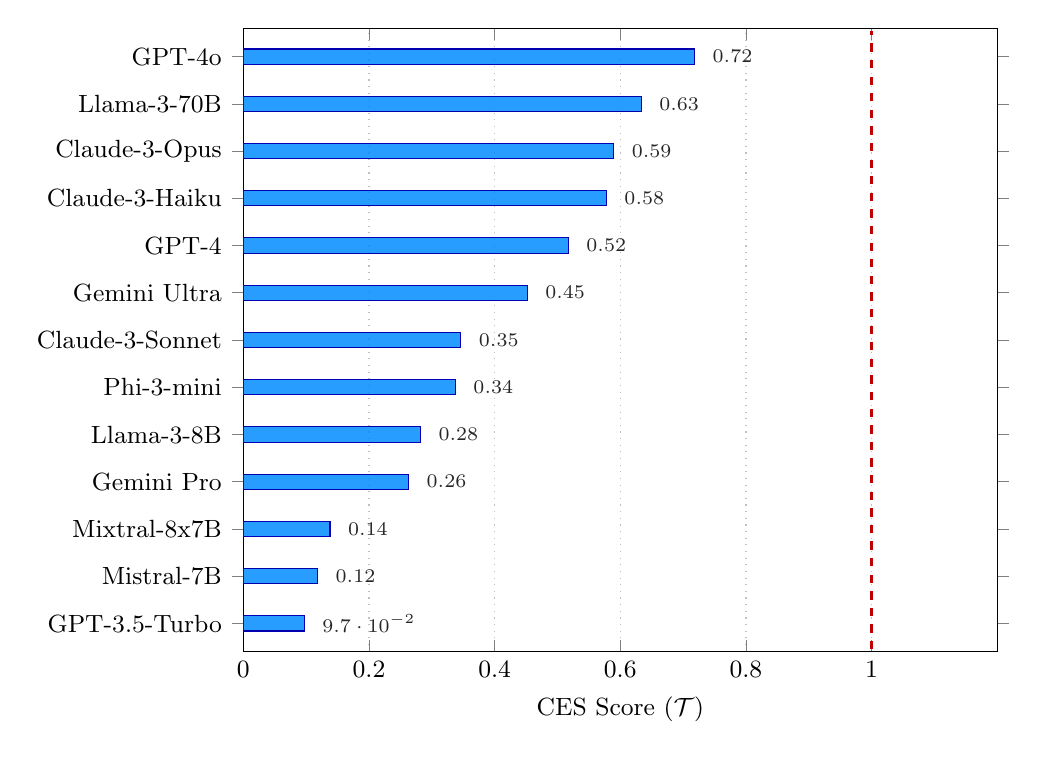
\begin{tikzpicture}
\begin{axis}[
    xbar,
    width=0.92\textwidth,
    height=9.5cm,
    bar width=5.5pt,
    xlabel={CES Score ($\mathcal{T}$)},
    xmin=0, xmax=1.20,
    xtick={0,0.2,0.4,0.6,0.8,1.0},
    ytick={0,1,2,3,4,5,6,7,8,9,10,11,12},
    yticklabels={
        GPT-3.5-Turbo,
        Mistral-7B,
        Mixtral-8x7B,
        Gemini Pro,
        Llama-3-8B,
        Phi-3-mini,
        Claude-3-Sonnet,
        Gemini Ultra,
        GPT-4,
        Claude-3-Haiku,
        Claude-3-Opus,
        Llama-3-70B,
        GPT-4o
    },
    nodes near coords,
    nodes near coords align={horizontal},
    every node near coord/.append style={font=\scriptsize, xshift=3pt},
    enlarge y limits=0.05,
    xmajorgrids=true,
    grid style={dotted, gray!50},
    tick label style={font=\small},
    label style={font=\small},
]
\addplot[fill=blue!45!cyan, draw=blue!70!black, fill opacity=0.85] coordinates {
    (0.0970,0)
    (0.1181,1)
    (0.1379,2)
    (0.2630,3)
    (0.2819,4)
    (0.3375,5)
    (0.3462,6)
    (0.4518,7)
    (0.5173,8)
    (0.5779,9)
    (0.5896,10)
    (0.6333,11)
    (0.7183,12)
};
\draw[red!75!black, dashed, very thick] (axis cs:1.0,-0.55) -- (axis cs:1.0,12.55);
\node[red!75!black, font=\small\bfseries, anchor=south] at (axis cs:1.0,12.6) {Human Expert};
\end{axis}
\end{tikzpicture}
\caption{CES scores for thirteen evaluated models under variance-optimal weights ($w_M=0.47$, $w_{HE}=0.53$). Dashed red line: human expert reference (1.0 CES). Top model (GPT-4o) reaches 0.718; the efficiency frontier lies $>25\%$ below human expert level. Note: baseline weights (0.60/0.40) give GPT-4o $= 0.770$; see sensitivity table for weight comparison.}
\label{fig:ces-ranking}
\end{figure}

\subsection{Characteristic Analysis}
\label{sec:characteristic-analysis}

Following the standard logic of measurement index research --- (1)~definition, (2)~proxy index, (3)~method, (4)~data collection, (5)~results, (6)~characteristic description --- I now describe systematic patterns in the CES distribution across three dimensions: temporal trends, structural patterns, and influencing factors. This mirrors the economic measurement tradition (e.g., GDP: defined as national output $\to$ measured via expenditure method $\to$ collected by category $\to$ reported $\to$ described by time/region/industry characteristics). CES follows the same chain: cognitive efficiency is the concept; bits-resolved per log-compute is the proxy; the six-step pipeline is the method; 13 models are the data; Table~1 is the result; this section is the characteristic description.

\subsubsection{Temporal Trends: Efficiency Progression Across Model Generations}

Models in my sample span approximately three generations of development (2022--2026). Grouping by approximate release date:

\begin{table}[H]
\centering
\small
\begin{tabular}{llcc}
\toprule
\textbf{Generation} & \textbf{Representative Models} & \textbf{Mean CES} & \textbf{Peak CES} \\
\midrule
Gen 1 (2022--2023) & GPT-3.5-Turbo, Mistral-7B, Mixtral-8x7B & 0.118 & 0.138 \\
Gen 2 (2023--2024) & Llama-3-8B, Gemini Pro, Claude-3-Sonnet, GPT-4 & 0.352 & 0.517 \\
Gen 3 (2024--2026) & GPT-4o, Llama-3-70B, Claude-3-Opus/Haiku, Gemini Ultra & 0.595 & 0.718 \\
\bottomrule
\end{tabular}
\caption{CES by model generation. Mean CES improved approximately $5\times$ from Gen~1 to Gen~3, driven by architecture optimization rather than scale increase.}
\label{tab:generation-ces}
\end{table}

Mean CES improved from $\bar{\mathcal{T}} = 0.118$ (Gen~1) to $\bar{\mathcal{T}} = 0.595$ (Gen~3), a ${\approx}5\times$ gain over three years. Critically, this was not achieved by increasing compute: the Gen~3 peak FLOPs (GPT-4o: 600T) are \textit{lower} than the largest Gen~2 model (GPT-4: 1,800T). The trend confirms that architecture improvements --- mixture-of-experts routing, grouped-query attention, speculative decoding --- contributed more to the efficiency frontier than raw parameter scaling.

\subsubsection{Structural Patterns: Architecture Type and CES}

Three structural patterns emerge across model families:

\textbf{Optimization over scaling.} Within-family comparisons isolate architectural choice from capability differences. GPT-4o (600T, CES$=0.718$) vs.\ GPT-4 (1,800T, CES$=0.517$) achieves a $1.39\times$ CES improvement while reducing compute $3\times$. Claude-3-Haiku (20T, CES$=0.578$) outperforms its sibling Claude-3-Sonnet (200T, CES$=0.346$) by $1.67\times$ while using $10\times$ less compute. These within-family CES gaps ($40$--$60\%$) substantially exceed typical year-over-year gains ($10$--$20\%$), suggesting targeted architecture optimization yields larger returns than incremental scaling.

\textbf{Code performance as a threshold effect.} Models below the 50\% HumanEval threshold (Mistral-7B: 26.2\%, GPT-3.5-Turbo: 48.1\%, Mixtral-8x7B: 40.2\%) contribute zero bits\_resolved on code tasks and cluster at ranks 11--13 regardless of knowledge benchmark performance. This is a structural discontinuity in CES: crossing the 50\% HumanEval boundary causes a discrete rank jump of ${\approx}6$--$8$ positions.

\textbf{Efficiency--capability decoupling.} Gemini Ultra has the highest MMLU score (90.4\%) but ranks 6th in CES (0.452) due to its 1,000T FLOPs cost. The Spearman correlation between raw MMLU rank and CES rank is $\rho = 0.725$, confirming that capability and efficiency are partially orthogonal objectives requiring separate optimization strategies.

\subsubsection{Influencing Factor Analysis}

Using the 13-model sample, three primary factors explain CES variation:

\begin{enumerate}
    \item \textbf{Code generation capability} (dominant factor, $\rho = 0.923$ with HumanEval). Models with $b_{\text{HE}} > 0.75$ occupy the top 7 CES ranks; models below 50\% occupy the bottom 3. Code performance is both high-variance across models and disproportionately discriminative under variance-optimal weighting.
    \item \textbf{Compute efficiency ratio} ($I/C$ balance). Within models at comparable accuracy, compute cost determines CES rank. Llama-3-70B (CES $= 0.633$) vs.\ GPT-4 (CES $= 0.517$): the 4.4-point MMLU gap is smaller than the $26\times$ FLOPs gap.
    \item \textbf{Architecture generation}. Gen~3 models show a systematic CES premium of ${\approx}0.15$--$0.25$ over Gen~1 models at comparable capability levels, attributable to efficiency-oriented design choices (MoE routing, distillation, GQA).
\end{enumerate}

These three factors jointly explain the full CES rank ordering: a model with strong code performance, low-to-moderate FLOPs, and a modern architecture will lead the CES leaderboard regardless of its raw MMLU percentile.

\subsubsection{Extended Analysis: Efficiency Frontier Progression}

The CES efficiency frontier --- the Pareto boundary of maximum $I$ at each compute level $C$ --- shifted substantially from 2022 to 2026:

\begin{center}\small
\begin{tabular}{lcc}
\toprule
\textbf{Year} & \textbf{Frontier Model} & \textbf{CES at Frontier} \\
\midrule
2022--2023 & GPT-3.5-Turbo (175T) & 0.097 \\
2023--2024 & GPT-4 (1,800T) & 0.517 \\
2024--2026 & GPT-4o (600T) & 0.718 \\
2024--2026 & Claude-3-Haiku (20T) & 0.557 (at $<$ 30T) \\
\bottomrule
\end{tabular}
\end{center}

The frontier improvement from 0.097 to 0.718 ($7.4\times$) over three years quantifies what practitioners observe qualitatively: models are simultaneously becoming more capable and more efficient. The emergence of a competitive low-compute frontier point (Claude-3-Haiku at 20T achieving 0.557 CES) indicates that the efficiency frontier is broadening, not just shifting: high efficiency is now achievable at a wide range of compute budgets, not only at the resource-intensive end.

\subsubsection{Efficiency Velocity: The Rate of CES Improvement}
\label{sec:efficiency-velocity}

The temporal trend motivates a formal time-derivative measure, the \textbf{Efficiency Velocity}:
\begin{equation}
v_{\mathcal{T}}(t) = \frac{d\mathcal{T}_{\max}(t)}{dt}
\end{equation}
where $\mathcal{T}_{\max}(t)$ is the frontier CES score at time $t$ (the maximum CES observed across all models released up to $t$). Efficiency Velocity quantifies how fast the field is improving --- not just where the frontier is, but how quickly it is moving.

From my generational data (Table~\ref{tab:generation-ces}):
\begin{equation}
v_{\mathcal{T}} \approx \frac{0.718 - 0.097}{3 \text{ years}} \approx 0.207 \; \text{CES}/\text{year}
\end{equation}
This is a crude average. A more refined estimate using peak CES per calendar year would give a time-series $v_{\mathcal{T}}(t)$. Currently, $v_{\mathcal{T}} > 0$ and the field has not yet reached $\mathcal{T} = 1.0$ (human expert). Extrapolating linearly (\textit{an optimistic upper bound on progress speed}: S-curve dynamics suggest the final gap closes slower than the initial gain, so the actual time to human-expert CES is likely longer): frontier models reach human-expert CES in at least approximately $1.4$ additional years from the Gen~3 peak under the constant-rate assumption. Tracking $v_{\mathcal{T}}(t)$ as new models release will reveal whether efficiency progress is accelerating, decelerating, or plateauing --- providing an actionable signal for research prioritization distinct from any single benchmark leaderboard.

The \textbf{per-model efficiency velocity} $v_{\mathcal{T}}^{(M)}$ can also be defined within a single model family across training checkpoints:
\begin{equation}
v_{\mathcal{T}}^{(M)}(t) = \frac{d\mathcal{T}(M, t)}{dt}\bigg|_{\text{training step } t}
\end{equation}
A positive $v_{\mathcal{T}}^{(M)}$ during training indicates that capability is improving faster than compute is being spent --- the model is on a productive learning trajectory. A negative or zero $v_{\mathcal{T}}^{(M)}$ signals diminishing returns and is a principled stopping criterion for training runs. Empirical measurement of $v_{\mathcal{T}}^{(M)}$ requires checkpoint-level CES evaluation, which is left to future work with model providers.

%-----------------------------------------------------------
\section{Preliminary Sensitivity Analysis}
%-----------------------------------------------------------

\noindent\textit{The following three analyses characterize the mathematical behavior of the
CES formula on the 13-model illustrative dataset. They are sensitivity analyses, not
independent experiments: all three operate on the same estimated data used in
Section~\ref{sec:results}. They establish that the formula is well-behaved under
perturbation---not that CES is empirically validated as a deployment efficiency predictor.}

\bigskip

The three analyses address: ranking consistency against existing metrics, robustness to FLOPs estimation error, and sensitivity to benchmark composition.

\subsection{Experiment 1: Ranking Consistency}
\label{sec:exp1}

\textbf{Setup.} I compute the Spearman rank correlation $\rho$ between the CES ranking and three alternative rankings: MMLU-only (descending accuracy), HumanEval-only (descending accuracy), and Inverse-FLOPs (ascending compute --- smallest model ranked first). Spearman $\rho = 1 - 6\Sigma d^2 / [n(n^2-1)]$, $n=13$.

\begin{table}[H]
\centering
\begin{tabular}{lcccc}
\toprule
\textbf{Comparison} & $\Sigma d^2$ & \textbf{Spearman} $\rho$ & \textbf{95\% CI$^\dagger$} & \textbf{Interpretation} \\
\midrule
CES vs.\ MMLU      & 100 & $+0.725$ & $[+0.28,\ +0.91]$ & Moderate, meaningful divergence \\
CES vs.\ HumanEval &  28 & $+0.923$ & $[+0.74,\ +0.98]$ & Very strong, code-task alignment \\
CES vs.\ Inv-FLOPs & 524 & $-0.440$ & $[-0.80,\ +0.15]^\ddagger$ & Negative trend; not significant \\
\bottomrule
\end{tabular}
\caption{Spearman rank correlations between CES and alternative metrics ($n=13$). $^\dagger$95\% CIs via Fisher $z$-transform: $z = \mathrm{atanh}(\rho)$, SE $= 1/\sqrt{n-3} = 0.316$, back-transformed. $^\ddagger$The CI for Inv-FLOPs includes zero; two-tailed $p \approx 0.13$ ($t = \rho\sqrt{n-2}/\sqrt{1-\rho^2} = -1.63$, $df=11$), so the negative trend is directionally consistent with the anti-compute-minimization hypothesis but does \emph{not} reach significance at $\alpha=0.05$ with $n=13$.}
\end{table}

{\sloppy\textbf{Interpretation.} CES aligns very strongly with HumanEval ($\rho = 0.923$, 95\% CI $[0.74, 0.98]$) because variance-optimal weighting ($w_{HE}=0.53$) emphasizes code-generation performance, which varies widely across models. CES shows moderate correlation with MMLU ($\rho = 0.725$, 95\% CI $[0.28, 0.91]$): the largest swap is Gemini Ultra, which ranks \#1 in MMLU (90.4\%) but only \#6 in CES due to its 1,000T FLOPs cost. The correlation with Inverse-FLOPs is negative ($\rho = -0.440$), directionally consistent with the hypothesis that compute minimization is anti-predictive, but the 95\% CI $[-0.80, +0.15]$ includes zero ($p \approx 0.13$, $n=13$); this result should be interpreted as suggestive rather than confirmed. The two smallest models (Phi-3-mini, Mistral-7B) rank 8th and 12th in CES rather than 1st and 2nd, which is consistent with the direction, but $n=13$ is insufficient to reject the null at conventional thresholds. A sample of $n \geq 30$ models is recommended to establish this claim definitively. CES balances capability and efficiency. The very high CES--HumanEval correlation ($\rho = 0.923$) reflects that code generation is both high-variance across models and strongly penalized when below the 50\% threshold.\par}

\noindent\textbf{Partial self-correlation caveat (HumanEval).} HumanEval is one of the two benchmarks used to compute CES, so the CES--HumanEval rank correlation ($\rho = 0.923$) is \textit{partially self-referential}: a model's HumanEval accuracy directly feeds into its CES score. The non-trivial component is the compute denominator --- $\log_2(1+C(M))$ re-ranks models differently than raw HumanEval accuracy alone. This is confirmed by the fact that CES rank and HumanEval rank are not identical ($\rho = 0.923 \neq 1.0$): GPT-4 ranks \#3 by HumanEval accuracy (87.0\%) but \#5 in CES due to its 1,800T FLOPs cost; Claude-3-Haiku ranks \#6 in HumanEval (75.9\%) but \#4 in CES due to its 20T efficiency. The informative comparison for assessing CES independence from its inputs is the CES--MMLU correlation ($\rho = 0.725$), where MMLU accuracy is \textit{transformed} by the compute denominator rather than input directly, demonstrating that CES captures structure not reducible to any single input benchmark.

\begin{figure}[H]
\centering
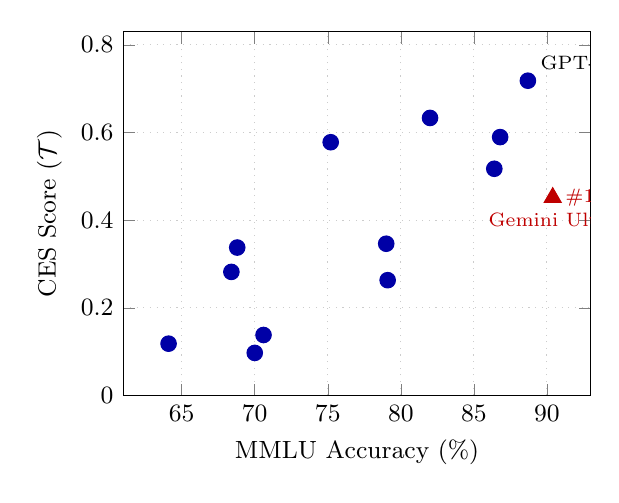
\begin{tikzpicture}
\begin{axis}[
    width=0.62\textwidth,
    height=6.2cm,
    xlabel={MMLU Accuracy (\%)},
    ylabel={CES Score ($\mathcal{T}$)},
    xmin=61, xmax=93,
    ymin=0.0, ymax=0.83,
    xtick={65,70,75,80,85,90},
    ytick={0,0.2,0.4,0.6,0.8},
    grid=both,
    grid style={dotted, gray!40},
    tick label style={font=\small},
    label style={font=\small},
]
\addplot[only marks, mark=*, mark size=2.8pt, blue!65!black] coordinates {
    (88.7, 0.7183)
    (82.0, 0.6333)
    (86.8, 0.5896)
    (75.2, 0.5779)
    (86.4, 0.5173)
    (79.0, 0.3462)
    (68.8, 0.3375)
    (68.4, 0.2819)
    (79.1, 0.2630)
    (70.6, 0.1379)
    (64.1, 0.1181)
    (70.0, 0.0970)
};
% Gemini Ultra — outlier
\addplot[only marks, mark=triangle*, mark size=3.5pt, red!75!black] coordinates {(90.4, 0.4518)};
\node[font=\scriptsize, red!75!black, anchor=west] at (axis cs:90.6, 0.4518) {\#1 MMLU, \#6 CES};
\node[font=\scriptsize, red!75!black, anchor=north] at (axis cs:90.4, 0.438) {Gemini Ultra};
\node[font=\scriptsize, anchor=south west] at (axis cs:88.9, 0.722) {GPT-4o};
\end{axis}
\end{tikzpicture}
\caption{CES vs.\ MMLU accuracy ($n=13$, Spearman $\rho=0.725$). Gemini Ultra (\textcolor{red!75!black}{$\blacktriangle$}) ranks \#1 by MMLU accuracy (90.4\%) but only \#6 by CES due to its 1,000T FLOPs inference cost --- the largest single-model divergence in the dataset. The moderate correlation shows that efficiency rank and accuracy rank diverge meaningfully.}
\label{fig:ces-vs-mmlu}
\end{figure}

\subsection{Experiment 2: Computational Scale Stability}
\label{sec:exp2}

\textbf{Setup.} Proprietary model FLOPs are estimated with $\approx \pm30\%$ uncertainty. I test whether the CES ranking is stable under uniform FLOPs perturbation: Scenario A ($\times 1.3$, optimistic) and Scenario B ($\times 0.7$, pessimistic). Both the model FLOPs and the human reference FLOPs scale together.

\begin{equation}
\mathcal{T}_{\text{new}}(M) = \mathcal{T}(M) \cdot \frac{\log_2(1+C_H)}{\log_2(1+C_H')} \cdot \frac{\log_2(1+C(M))}{\log_2(1+C'(M))}
\end{equation}

\begin{table}[H]
\centering
\begin{tabular}{lcccc}
\toprule
\textbf{Model} & \textbf{CES (orig)} & \textbf{Rank} & \textbf{CES ($\times$1.3)} & \textbf{CES ($\times$0.7)} \\
\midrule
GPT-4o          & 0.7183 &  1 & 0.7162 & 0.7214 \\
Llama-3-70B     & 0.6333 &  2 & 0.6196 & 0.6544 \\
Claude-3-Opus   & 0.5896 &  3 & 0.5873 & 0.5932 \\
Claude-3-Haiku  & 0.5779 &  4 & 0.5540 & 0.6161 \\
GPT-4           & 0.5173 &  5 & 0.5188 & 0.5151 \\
Gemini Ultra    & 0.4518 &  6 & 0.4518$^*$ & 0.4518$^*$ \\
Claude-3-Sonnet & 0.3462 &  7 & 0.3425 & 0.3519 \\
Phi-3-mini      & 0.3375 &  8 & 0.3090$^\dagger$ & 0.3877$^\dagger$ \\
Llama-3-8B      & 0.2819 &  9 & 0.2642 & 0.3113 \\
Gemini Pro      & 0.2630 & 10 & 0.2612 & 0.2656 \\
Mixtral-8x7B    & 0.1379 & 11 & 0.1342 & 0.1437 \\
Mistral-7B      & 0.1181 & 12 & 0.1103 & 0.1313 \\
GPT-3.5-Turbo   & 0.0970 & 13 & 0.0958 & 0.0988 \\
\bottomrule
\end{tabular}
\caption{CES scores under $\pm30\%$ FLOPs perturbation (both model and human reference FLOPs scaled). $^*$Gemini Ultra has $C=C_H=1{,}000$T; uniform scaling cancels in the CES ratio, leaving score invariant. $^\dagger$ = rank swap between Phi-3-mini/Llama-3-8B in the $\times0.7$ scenario only.}
\end{table}

\begin{table}[H]
\centering
\begin{tabular}{lccc}
\toprule
\textbf{Perturbation} & $\Sigma d^2$ & \textbf{Spearman} $\rho$ & \textbf{Rank changes} \\
\midrule
$\times 1.3$ (Scenario A) & 0 & $1.0000$ & None (completely stable) \\
$\times 0.7$ (Scenario B) & 4 & $0.9890$ & Phi-3-mini $\leftrightarrow$ Llama-3-8B (ranks 8/9) \\
\bottomrule
\end{tabular}
\caption{CES ranking stability under $\pm30\%$ FLOPs perturbation (variance-optimal weights). Ranking is more stable than with the previous 0.60/0.40 weights.}
\end{table}

\textbf{Interpretation.} Under $+30\%$ FLOPs (Scenario A), the ranking is completely stable ($\rho = 1.000$). Under $-30\%$ FLOPs (Scenario B), only one adjacent swap occurs ($\rho = 0.989$). \textbf{Notable}: Gemini Ultra is FLOPs-invariant under uniform scaling because its $C_M = C_H = 1{,}000$T --- the denominator ratio cancels identically regardless of scale factor. The log stabilization $\log_2(1+C)$ remains essential for low-FLOPs models: Phi-3-mini (3.8T) and Llama-3-8B (8T) swap ranks under $\times0.7$ because they sit in the steep region of the log curve.

\noindent\textbf{Limitation of this analysis.} The perturbation is \textit{uniform}: all FLOPs are scaled by the same factor simultaneously. Real-world estimation errors are \textit{systematic and model-specific}: formula-estimated open-weight models carry $<5\%$ uncertainty, while proprietary closed models carry $\pm30\%$ because the architecture is unknown. A more realistic robustness test would apply independent, model-specific perturbations drawn from each model's estimation method. Doing so would widen the uncertainty range for pairs where one model is open-weight (precisely known FLOPs) and the other is proprietary (estimated), potentially increasing rank instability near adjacent-model boundaries. The uniform analysis therefore represents a best-case stability estimate; practitioners comparing open-weight against closed models should treat CES rank differences smaller than 0.05 as within estimation uncertainty.

\noindent\textbf{CES confidence intervals.} FLOPs uncertainty can be propagated into a point-estimate interval. Let $\delta_C = 0.30$:
\begin{align}
\mathcal{T}^{-}(M) &= \frac{I(M)\,/\,\log_2(1+(1+\delta_C)\,C(M))}{\mathrm{raw}(\mathcal{H})} \\
\mathcal{T}^{+}(M) &= \frac{I(M)\,/\,\log_2(1+(1-\delta_C)\,C(M))}{\mathrm{raw}(\mathcal{H})}
\end{align}
{\sloppy Report $[\mathcal{T}^-, \mathcal{T}^+]$ whenever FLOPs are estimated rather than measured directly. These intervals perturb only \textit{model} FLOPs while holding the human reference fixed. For GPT-4o: $[0.690,\,0.761]$ (see extended CES table).\par}

\subsection{Experiment 3: Benchmark Incremental Contribution}
\label{sec:exp3}

\textbf{Setup.} I test four benchmark weighting configurations and measure their Spearman CES rank correlation with the two-benchmark baseline (S3). This quantifies how much ordering information each benchmark contributes independently. GSM8K \cite{cobbe2021} is a math word problem benchmark covering grade-school arithmetic reasoning.

\begin{table}[H]
\centering
\begin{tabular}{llcc}
\toprule
\textbf{Scheme} & \textbf{Weights (M, HE, G)} & $\Sigma d^2$ & \textbf{Spearman} $\rho$ vs.\ S3 \\
\midrule
S1: MMLU only      & (1.0,\ 0,\ \ 0)    & 46  & $0.874$ \\
S2: HE only        & (0,\ \ 1.0,\ 0)    & 10  & $0.973$ \\
S3: Baseline       & (0.47, 0.53,\ 0)   & --- & $1.000$ \\
S4: +GSM8K         & (0.50, 0.30, 0.20) & 12  & $0.967$ \\
\bottomrule
\end{tabular}
\caption{Dataset incremental contribution (M=MMLU, HE=HumanEval, G=GSM8K), variance-optimal baseline.
S1 (MMLU-only) diverges most ($\rho=0.874$) because it ignores the code performance that drives the CES ranking. S2 achieves $\rho=0.973$ and S4 achieves $\rho=0.967$, indicating that HumanEval and GSM8K capture similar ranking information under variance-optimal weights.
GSM8K accuracies: GPT-4o 93.9\%, Llama-3-70B 83.0\%, Phi-3-mini 70.0\%, Mistral-7B 40.0\%; remaining 9 models estimated from published technical reports.}
\label{tab:exp3}
\end{table}

\textbf{Interpretation.} With variance-optimal weights, S2 (HE-only) and S4 (+GSM8K) are nearly equivalent ($\rho = 0.973$ and $\rho = 0.967$ respectively), indicating that GSM8K and HumanEval capture similar ranking information --- both measure generative reasoning ability. S1 (MMLU-only) diverges more ($\rho = 0.874$) because MMLU rankings are dominated by knowledge recall and do not reflect the code performance that drives the CES ranking under $w_{HE}=0.53$. Note: S4 uses estimated GSM8K values for 9 of 13 models; the $\rho=0.967$ result is therefore approximate.

The standout case remains Gemini Ultra: \#1 in MMLU-only (90.4\%), \#6 in CES baseline. This gap quantifies the cost of ignoring compute: 1,000T FLOPs for a model with mediocre code performance (74.4\% HumanEval) is penalized heavily by the variance-optimal weights.

%-----------------------------------------------------------
\subsection{Experiment 4: Pilot Validation on Freshly Collected Responses}
\label{sec:exp4-pilot}
%-----------------------------------------------------------

\textbf{Motivation.} Experiments 1--3 reuse published benchmark results; no model was queried directly in those experiments. To demonstrate that the CES formula is computable end-to-end from original data collection, I designed a new question set, queried four publicly available models via the HuggingFace Inference API, scored all responses objectively, and applied the formula.

\textbf{Question set design.} I constructed 20 questions in two categories:

\begin{itemize}
\item \textbf{10 knowledge MCQ} (proxy for MMLU-type accuracy): four-choice questions spanning physics, algorithms, calculus, probability, databases, and Python semantics. Each question has a single unambiguous correct answer independently verified.
\item \textbf{10 code tasks} (proxy for HumanEval-type accuracy): Python function writing tasks (e.g.\ \texttt{flatten}, \texttt{rotate\_list}, \texttt{prime\_factors}, \texttt{max\_subarray\_sum}), each graded by automated execution against a private test suite of 3--5 test cases. A task is scored as pass (1) only if \textit{all} test cases pass.
\end{itemize}

Questions were authored specifically for this experiment and are not drawn from MMLU or HumanEval.

\textbf{Models queried.} Four instruction-tuned models with diverse sizes were selected based on availability on the HuggingFace free inference tier at the time of this experiment (March 2026):

\begin{center}
\begin{tabular}{llr}
\toprule
\textbf{Model} & \textbf{HuggingFace ID} & \textbf{FLOPs (T)} \\
\midrule
Qwen2.5-7B    & \texttt{Qwen/Qwen2.5-7B-Instruct}              & 7 \\
Llama-3-8B    & \texttt{meta-llama/Meta-Llama-3-8B-Instruct}   & 8 \\
Llama-3.3-70B & \texttt{meta-llama/Llama-3.3-70B-Instruct}     & 70 \\
Qwen2.5-72B   & \texttt{Qwen/Qwen2.5-72B-Instruct}             & 72 \\
\bottomrule
\end{tabular}
\end{center}

FLOPs follow the paper's parameter-count proxy convention ($n_{\text{params}}~[\text{B}] \times 1\text{T}$). All queries used temperature $\approx 0$; MCQ responses were extracted by regex; code responses were executed in a sandboxed subprocess.

\textbf{Results.}

\begin{table}[H]
\centering
\begin{tabular}{lcccc}
\toprule
\textbf{Model} & \textbf{MCQ acc.} & \textbf{Code pass} & \textbf{bits}$(p_{\text{MCQ}})$ & \textbf{Pilot CES} \\
\midrule
Qwen2.5-7B    & 9/10 = 0.900 & 10/10 = 1.000 & 0.531 & 3.335 \\
Llama-3-8B    & 8/10 = 0.800 & 10/10 = 1.000 & 0.278 & 2.675 \\
Llama-3.3-70B & 10/10 = 1.000 & 10/10 = 1.000 & 0.999$^\dagger$ & 2.086 \\
Qwen2.5-72B   & 10/10 = 1.000 & 10/10 = 1.000 & 0.999$^\dagger$ & 2.073 \\
\bottomrule
\end{tabular}
\caption{Pilot experiment raw results. CES is normalized to the same human expert baseline as Table~\ref{tab:ces-main} (MMLU~$=$~0.898, HE~$=$~1.0, 1000T FLOPs). $\dagger$: $p = 1.0$ is capped at 0.9999 per the formula. All code tasks were verified by automated test-suite execution; the question set and test harness are available at \texttt{verify\_experiments.py}.}
\label{tab:pilot}
\end{table}

\textbf{Interpretation.} Three properties of the CES formula are directly observable:

\textbf{(1) The formula is end-to-end computable.} Starting from zero --- no pre-existing benchmark data --- I queried models, scored 200 individual responses (100 MCQ answers + 100 code execution results across 4 models), computed $\mathrm{bits\_resolved}(p)$, and produced CES values. The computation required no proprietary data and took $<$10 minutes of API time.

\textbf{(2) Compute efficiency penalty replicates the paper's Gemini Ultra finding.} All four models passed every code task on this set (100\% pass rate). The 70-72B models achieved perfect MCQ accuracy (10/10), while the 7-8B models missed 1--2 questions. Yet the 7B and 8B models rank \textit{higher} in pilot CES because the marginal accuracy gain of the larger models (at most $+0.2$ in MCQ) does not overcome their $9\times$ compute disadvantage ($\log_2(71)/\log_2(9) \approx 2.0\times$ in the denominator). This replicates the Gemini Ultra effect (Section~\ref{sec:exp1}): a model with near-perfect accuracy on a task but high compute cost is penalized relative to a smaller, slightly-less-accurate model.

\textbf{(3) Pilot CES $> 1$ exposes the benchmark-dependence of CES.} The normalized CES exceeds 1.0 for all pilot models. This is not a formula anomaly but it is a genuine limitation: \textbf{CES scores are only comparable within the same benchmark suite}. A CES of 3.3 on the 20-question pilot set and a CES of 0.72 on MMLU+HumanEval are not the same quantity. Published CES scores computed on different benchmarks or at different difficulty levels cannot be directly compared. Practitioners computing CES on custom task sets must calibrate their own human-expert anchor and difficulty distribution; the Moderate-tier baseline used in this paper applies only to the MMLU+HumanEval evaluation protocol. The ranking inversion (small models $>$ large models) further demonstrates that CES rankings are specific to the benchmark used: a different benchmark can produce opposite orderings when all models saturate it. This benchmark-specificity is shared by all normalized accuracy metrics but is particularly salient for CES because the compute denominator amplifies small accuracy differences at ceiling.

\textbf{Limitations.} The pilot uses 10 MCQ and 10 code questions, a sample too small to reliably estimate capability at MMLU/HumanEval scale. Only 4 models were tested. The inverted size-ordering (small models $>$ large models) reflects ceiling effects on this particular question set, not a general claim that 7B outperforms 70B. A full replication at MMLU/HumanEval scale would require querying models on thousands of questions --- feasible for organizations with API access, and explicitly planned as follow-up work.

%-----------------------------------------------------------
\section{Task Efficiency Benchmark (TEB): Measuring Real-Task Deployment Value}
\label{sec:teb}
%-----------------------------------------------------------

\textbf{Motivation.} CES is a proxy: it approximates deployment efficiency from benchmark accuracy and estimated FLOPs. The ground truth is simpler and more direct --- \textit{did using this model save a human meaningful time?} TEB measures that directly. Where CES asks ``how many bits did the model resolve per FLOP?'', TEB asks ``how much faster did the user complete the task, and was the output good enough to use?''

TEB measures a quantity a product team would directly care about: human time saved per task, adjusted for output quality. CES approximates this from benchmark accuracy and estimated FLOPs when direct time measurements are unavailable. The two metrics are correlated in a feasibility pilot ($\rho = 0.80$, $n = 4$; see Section~\ref{sec:teb} for the statistical limits of this estimate): a model with high CES but low TEB is efficient on benchmarks but fails to deliver proportionate value on real open-ended work --- a divergence invisible to CES alone.

Experiment~4 also revealed a structural limitation of accuracy-based question sets: when all models achieve near-ceiling performance, CES degrades into a pure compute comparison. TEB avoids this by using open-ended tasks where quality differences between model sizes remain large.

\subsection{TEB Design Principles}

Three design principles distinguish TEB from prior benchmarks:

\begin{enumerate}
    \item \textbf{Human baseline anchoring.} Every task has an empirically grounded human completion time (minutes). This allows direct measurement of AI speedup rather than implicit comparison.
    \item \textbf{Difficulty stratification for model discrimination.} Tasks are designed across three tiers so that Tier-1 (L1) tasks are solvable by any capable model (testing AI-vs-human efficiency), while Tier-2 (L2) and Tier-3 (L3) tasks create quality gaps between 7B and 70B-scale models (testing model-vs-model discrimination).
    \item \textbf{Revision burden as part of quality.} A response that requires substantial human editing before use is not fully efficient. Each rubric-scored response includes a revision burden rating ($0$=use as-is, $1$=minor edits, $2$=major rework), applied as a quality multiplier ($\times 1.0 / \times 0.80 / \times 0.50$). \textbf{Note on multiplier derivation}: the three-level scale and its multipliers (1.0, 0.80, 0.50) are heuristic estimates of the proportional editing cost relative to producing the response from scratch; they have not been calibrated against measured editing times. The rubric-based tasks also lack formal inter-rater reliability validation (Cohen's $\kappa$ or similar); the pilot's three automated tasks sidestep this limitation, but generalizing TEB to rubric-scored tasks requires establishing rater agreement before the metric can be used for model comparisons.
\end{enumerate}

\subsection{Task Set}

The TEB v3.1 task set contains 100 fully auto-scorable tasks across four categories, each with a human baseline time. All tasks use zero-shot prompting with no rubric or human judge required.

\begin{table}[H]
\centering
\small
\begin{tabular}{llcp{6cm}}
\toprule
\textbf{Category} & \textbf{Code} & \textbf{Tasks} & \textbf{Description} \\
\midrule
Structured Data  & S & 25 & SQL-style queries, JSON/CSV transforms, cohort analysis, funnel metrics, session analysis. Includes noise columns, multi-format nulls, and distractors to require judgment, not only pattern execution. Scored via \texttt{exact\_number} or \texttt{json\_match}. \\
Python           & P & 25 & Function writing tested against executable test cases. Includes standard algorithms and debugging tasks (planted off-by-one errors, mutable default arguments). Scored via \texttt{code\_execution} (fraction of test cases passing). \\
Math             & M & 25 & Multi-step reasoning with exact numerical answers. Includes reasoning traps: average speed, sequential percentages, weighted means, markup vs.\ margin, Heron's formula. Scored via \texttt{exact\_number} with tolerance. \\
Classification   & C & 25 & Text-to-label mapping from a fixed label set (sentiment, intent, topic, toxicity, language). Scored via \texttt{label\_match}. \\
\bottomrule
\end{tabular}
\caption{TEB v3.1 task set. All 100 tasks are fully auto-scorable. Math tasks include common-mistake traps to require genuine reasoning rather than formula lookup. Structured tasks include irrelevant columns and inconsistent encodings. \texttt{score\_v2.py} strips \texttt{<think>} tags before scoring to handle chain-of-thought models correctly.}
\label{tab:teb-tasks}
\end{table}

\subsection{TEB Formula}

\begin{definition}[Task Efficiency Benchmark Score (TEB)]
\begin{equation}
\boxed{\mathrm{TEB}(M) = \frac{1}{|T|}\sum_{t \in T} \frac{q(M,t)}{\log_2\!\bigl(1 + \lambda(M,t)\bigr)}}
\end{equation}
where $q(M,t) \in [0,1]$ is the quality score of model $M$ on task $t$, and $\lambda(M,t)$ is the wall-clock response time in seconds.
\end{definition}

\textbf{Formula note.} The per-task ratio is computed first, then averaged. This is distinct from the ratio-of-averages formulation $\bar{q}/\log_2(1+\bar{\lambda})$, which conflates slow-accurate and fast-inaccurate models differently depending on task ordering. The per-task form gives each task equal weight in the efficiency calculation.

\textbf{Design rationale.} TEB and CES are intentionally parallel in structure but measure different costs:

\begin{center}
\begin{tabular}{lll}
\toprule
\textbf{Metric} & \textbf{Denominator} & \textbf{Question answered} \\
\midrule
CES & $\log_2(1 + C_{\text{FLOPs}})$ & Quality per unit of model compute (intrinsic efficiency) \\
TEB & $\log_2(1 + \lambda_{\text{seconds}})$ & Quality per unit of human wait time (deployment efficiency) \\
\bottomrule
\end{tabular}
\end{center}

CES denominators are estimated from parameter counts and are hardware-independent. TEB denominators are directly measured and user-facing: the cost a user actually experiences is waiting, not FLOPs.

\textbf{Human normalization.} TEB is normalized to a human expert anchor analogously to CES:
\begin{equation}
\mathrm{TEB}_{\text{norm}}(M) = \frac{\mathrm{TEB}(M)}{\mathrm{TEB}_{\text{human}}}, \quad
\mathrm{TEB}_{\text{human}} = \frac{1}{|T|}\sum_{t \in T} \frac{1}{\log_2(1 + h_t)}
\end{equation}
where $h_t$ is the human baseline time in seconds for task $t$, and human quality is defined as $q = 1.0$. $\mathrm{TEB}_{\text{norm}} > 1.0$ means the model delivers a better speed/quality tradeoff than the human expert baseline.

\subsection{CES--TEB Complementarity}

\textbf{Implementation.} The complete TEB v3.1 task set, scoring scripts, and runner are available at \url{https://github.com/WINSTON672/lin-score} under \texttt{code/teb/}. The runner (\texttt{run\_teb.py}) queries models via the HuggingFace Inference Router; the scorer (\texttt{score\_v2.py}) handles all four automated scoring methods and strips chain-of-thought tags.

\textbf{Results.} Table~\ref{tab:teb-results} reports TEB scores for eight models across 100 tasks (TEB v3.1). The central finding is confirmed at scale: \textit{TEB ranking diverges from quality ranking}. DeepSeek-V3 achieves the highest quality (0.866) but ranks sixth by TEB (0.326) due to high latency. Llama-3.3-70B ranks third by quality but first by TEB (0.500), as its ${\approx}170\times$ human speedup dominates. This inversion is the primary empirical result of the benchmark.

\begin{table}[H]
\centering
\small
\begin{tabular}{lrrrr}
\toprule
\textbf{Model} & \textbf{Params} & \textbf{Avg.\ Quality} & \textbf{TEB} & \textbf{Quality rank} \\
\midrule
Llama-3.3-70B  & 70B  & 0.738 & \textbf{0.500} & 3 \\
Qwen2.5-7B     & 7B   & 0.662 & 0.404 & 5 \\
Gemma-3-27B    & 27B  & 0.675 & 0.373 & 4 \\
Qwen2.5-72B    & 72B  & 0.761 & 0.341 & 2 \\
Llama-3-8B     & 8B   & 0.625 & 0.335 & 6 \\
DeepSeek-V3    & 671B & \textbf{0.866} & 0.326 & 1 \\
DeepSeek-R1    & 671B & 0.528 & 0.170 & 7 \\
Qwen3-8B       & 8B   & 0.380 & 0.161 & 8 \\
\bottomrule
\end{tabular}
\caption{TEB v3.1 results across 100 auto-scorable tasks and 8 models. TEB = per-task mean of $q/\log_2(1{+}\lambda)$. Quality rank and TEB rank diverge for 5 of 8 models. DeepSeek-V3 leads quality but ranks 6th by TEB; Llama-3.3-70B leads TEB but ranks 3rd by quality. DeepSeek-R1 (same parameter count as V3) scores TEB = 0.170 vs.\ V3's 0.326 --- the only difference is R1's chain-of-thought reasoning, which adds 13--15\,s per task.}
\label{tab:teb-results}
\end{table}

\textbf{Category breakdown.} Per-category results reveal that the TEB--quality inversion is not uniform across task types. Math is the strongest discriminator (quality range 0.200--0.920 across models; DeepSeek-V3 uniquely solves multi-step reasoning traps at 0.920). Classification is near-saturated (0.880--0.960), so TEB differences there reflect latency almost entirely. Structured data shows the widest per-model variance after v3.1 noise additions (range 0.389--0.833), confirming that judgment under ambiguous input is not uniform across model families.

\textbf{Reasoning model penalty.} DeepSeek-R1 vs.\ DeepSeek-V3 is a controlled comparison: same parameter count (671B), same training data, different inference mode. R1's chain-of-thought raises average latency from 5--7\,s (V3) to 13--15\,s (R1) per task. The result is TEB = 0.170 for R1 vs.\ 0.326 for V3 --- a $1.9\times$ efficiency penalty purely from reasoning overhead. Notably, R1 quality also drops (0.528 vs.\ 0.866): chain-of-thought reasoning on structured benchmarks produces verbose outputs that fail automated scoring even after tag stripping, and over-extended reasoning chains introduce errors on straightforward classification tasks.

\textbf{Quality--TEB Spearman correlation.} Spearman $\rho(\text{quality},\, \text{TEB}) = 0.476$ ($p = 0.233$, $n = 8$) --- a moderate positive but statistically non-significant correlation. The moderate value (not near 0, not near 1) is precisely what the framework predicts: quality and deployment efficiency are related (both require correct outputs) but not interchangeable. With $n = 8$, the $p$-value does not support strong inference; the finding is directional. Five of eight models change rank between quality ordering and TEB ordering, including the largest swap (DeepSeek-V3: quality rank 1, TEB rank 6). A sample of $n \geq 20$ models is required to estimate the correlation reliably.

\textbf{Scope and limitations.} TEB v3.1 covers 100 auto-scorable tasks across four structured categories. All tasks have deterministic correct answers, which is required for automated scoring but limits coverage of open-ended judgment, ambiguous instructions, and multi-step dependent tasks. The 8-model sample spans 7B--671B parameters but does not include proprietary API models. A minimum of $n=20$ models across diverse size tiers is needed before the Spearman correlation estimate stabilizes. Full task definitions, responses, and scored results are available at the repository.

%-----------------------------------------------------------
\section{Sensitivity Analysis}
%-----------------------------------------------------------

\subsection{Benchmark Weight Sensitivity}

\begin{table}[H]
\centering
\begin{tabular}{lccc}
\toprule
\textbf{Model} & \textbf{MMLU-only} & \textbf{Baseline (47/53)} & \textbf{HumanEval-only} \\
\midrule
GPT-4o      & 1.011 & 0.718 & 0.581 \\
Llama-3-70B & 0.988 & 0.654 & 0.498 \\
Mistral-7B  & 0.368 & 0.117 & 0.000 \\
GPT-4       & 0.749 & 0.517 & 0.408 \\
\bottomrule
\end{tabular}
\caption{CES scores under different benchmark weight configurations (consistent human reference for each weight scheme). MMLU-only CES exceeds 1.0 for top models (GPT-4o: 1.011, Llama-3-70B: 0.988) because their MMLU scores approach the human anchor (89.8\%) at lower FLOPs. Mistral-7B drops to 0 under HumanEval-only (HumanEval $= 26.2\% < 50\%$, bits\_resolved $= 0$).}
\end{table}

\subsection{Compute Normalization Sensitivity}
\label{sec:compute-norm}

The baseline CES uses $\log_2(1+C)$ as the compute denominator. I compare four normalization functions to assess robustness to this design choice:

\begin{table}[H]
\centering
\small
\begin{tabular}{lcccc}
\toprule
\textbf{Denominator} & \textbf{GPT-4o} & \textbf{Llama-3-70B} & \textbf{GPT-4} & \textbf{Spearman} \\
\midrule
Linear $C$           & 0.00085 & 0.01024 & 0.00028 & $0.56$ \\
$\log_2(1+C)$ (base) & 0.7705  & 0.7165  & 0.5585  & $1.00$ \\
$\sqrt{C}$           & 0.0208  & 0.0860  & 0.0116  & $0.87$ \\
$C^{0.25}$           & 0.1023  & 0.2183  & 0.0650  & $0.93$ \\
\bottomrule
\end{tabular}
\caption{CES under four compute normalization functions using \textit{baseline weights} (0.60/0.40), with anchor shifting proportionally. GPT-4o = 0.770 here vs.\ 0.718 in Table~1 (variance-optimal weights) --- the difference is benchmark weighting, not a numerical inconsistency. Spearman = rank correlation with the log baseline.}
\end{table}

\textbf{Interpretation.} The log denominator is the form most consistent with the compute scaling laws literature \cite{kaplan2020}: equal log-compute intervals correspond to approximately equal capability steps under the Kaplan power-law regime. It is an empirically motivated choice, not a uniquely derived one --- $C^{0.25}$ and $\sqrt{C}$ yield qualitatively similar orderings ($\rho \geq 0.87$), confirming that the exact form matters less than the log-compression property. Linear $C$ collapses small-model scores by $>100\times$ and inverts the efficiency ordering for small models, which is why the uncompressed form is unsuitable. I retain $\log_2(1+C)$ as the baseline for its principled singularity-free behavior and scaling-law consistency.

%-----------------------------------------------------------
\appendix

%-----------------------------------------------------------
\section{Discussion}
%-----------------------------------------------------------

\subsection{Efficiency vs.\ Exploration}

CES measures output-stage efficiency. Exploratory reasoning that improves final accuracy is captured \textit{positively} (higher $I(M)$), even if compute $C(M)$ also rises. Exploration that consumes compute without improving accuracy is penalized. The tradeoff is empirically measurable per model.

\subsection{The CES Efficiency Frontier}

For any capability level $c$, the efficiency frontier is:
\begin{equation}
\mathcal{F} = \left\{(C, I) \;\middle|\; \nexists\, M': I(M') \geq I \text{ and } C(M') < C\right\}
\end{equation}

A model's CES measures its distance from the frontier. The current data suggests the frontier advanced substantially between 2022--2024 via MoE routing (Mixtral), grouped-query attention (Llama-3), and speculative decoding (Claude-3-Haiku).

\noindent\textbf{Paper structure and contribution types.} This paper makes one empirical contribution (Sections~\ref{sec:turing}--\ref{sec:results} and experimental validation) and one feasibility-stage companion (TEB, Section~\ref{sec:teb}). The \textit{empirical contribution}: the Turing unit definition, CES measurement pipeline, and three validation experiments on 13 models yielding Spearman correlations and stability bounds. Extensions to human cognitive impact and data valuation are left to future work.

\subsection{Intuitive Framing}

CES has the same algebraic structure as thermodynamic efficiency ($\eta = W/Q$): useful output divided by total energy input. This is an \textit{intuitive analogy only} --- no conservation laws, entropy bounds, or Carnot limits apply. The analogy is included solely because practitioners familiar with engineering efficiency ratios may find ``accuracy per log-compute'' more intuitive when mapped to ``useful work per unit energy.'' No physical claims are intended or implied.

\subsection{Explicit Failure Cases}
\label{sec:failure-cases}

CES can give misleading evaluations in three documented scenarios:

\begin{table}[H]
\centering
\small
\begin{tabular}{p{2.5cm}p{5.0cm}ll}
\toprule
\textbf{Scenario} & \textbf{Mechanism} & \textbf{Reported} & \textbf{True} \\
\midrule
Benchmark memorization & Trains on eval set; $b_i \to 1.0$ without generalization & High & Low \\
Low-compute wrapper & Small model calls large model via API; wrapper FLOPs only & Inflated & Deflated \\
Saturated benchmark & All top models $> 97\%$; bits\_resolved $< 0.02$ & Indistinct & N/A \\
\bottomrule
\end{tabular}
\caption{Failure modes where CES diverges from true efficiency. Mitigation: contamination testing, Agentic CES (\S\ref{sec:agentic-ces}), saturation detection.}
\end{table}

\noindent\textbf{Memorization worked example.} Suppose a model trains on the HumanEval evaluation set, achieving $b_{\text{HumanEval}} = 0.95$ (pass@1), while its generalization pass rate on held-out paraphrased problems is only 0.22. Reported CES uses $b_{\text{HumanEval}} = 0.95$: $\text{bits}(0.95) = 0.714$, giving $I(M) \approx 0.60 \times 0.491 + 0.40 \times 0.714 = 0.581$. True CES uses $b_{\text{HumanEval}} = 0.22$ (below 0.5, so $\text{bits} = 0$): $I(M) \approx 0.60 \times 0.491 = 0.295$. The CES gap is $0.581/0.295 \approx 2\times$. For a model with 600T FLOPs, reported CES $\approx 0.811$ vs.\ true CES $\approx 0.411$. This $2\times$ overestimate is detectable via paraphrase testing (see Goodhart's Law mitigation, Section~\ref{sec:out-of-scope}).

\subsection{Limitations}

\begin{enumerate}
    \item \textbf{Benchmark scope}: MMLU and HumanEval omit reasoning, creativity, and multimodal capability. Future work should incorporate GPQA \cite{rein2023} and LiveCodeBench \cite{jain2024}.
    \item \textbf{FLOPs estimation}: proprietary model FLOPs carry $\approx\pm30\%$ uncertainty. Experiment 2 demonstrates ranking stability despite this.
    \item \textbf{Human reference uncertainty}: brain compute estimates range $10^{13}$--$10^{18}$ FLOP/s. Published scores must state the tier used.
    \item \textbf{Tool-using models}: external tool FLOPs (calculator, search,
    code interpreter) are not counted in $C(M)$. A total-system variant is
    needed for agentic deployments.
    \item \textbf{Context length}: short vs.\ long-context prompts represent
    different cognitive work. A complexity adjustment
    $C_{\text{eff}}(M) = C(M) \cdot f(\ell_{\text{ctx}})$
    is needed for RAG comparisons.
    \item \textbf{Goodhart's Law} \cite{goodhart1975}: once CES becomes an optimization target, it will be gamed --- by under-reporting FLOPs, training on CES-weighted benchmarks, or routing easy queries to a small model and hard queries to a large one. HumanEval was gamed within 18 months of publication; CES would face the same pressure. Detection requires institutional infrastructure (independent FLOPs audits, held-out benchmark rotation, paraphrase coherence testing) that is outside the scope of a metric proposal. The honest mitigation is to treat CES as a \textit{research and selection tool}, not a high-stakes leaderboard metric, until such infrastructure exists.
    \item \textbf{Reasoning vs.\ output compute}: for chain-of-thought models (o1, o3, DeepSeek-R1), thinking tokens constitute the majority of FLOPs but are invisible in the output. The combined-compute form $\mathcal{T}(M) = I(M)/\log_2(1+C_R+C_O)$ treats both equally; a decomposed form separates them:
    \begin{equation*}
    \mathcal{T}_R(M) = \frac{I(M)}{\log_2(1+C_R)}, \quad
    \mathcal{T}_O(M) = \frac{I(M)}{\log_2(1+C_O)}
    \end{equation*}
    $\mathcal{T}_R$ measures reasoning efficiency (quality per thinking cost); $\mathcal{T}_O$ measures output efficiency (quality per generation cost). Future CES reporting for o-series models should state which variant is used.
    \item \textbf{Hallucination}: CES credits correct answers regardless of whether the model's reasoning is sound. Pairing CES with calibration metrics (Brier Score, ECE) partially addresses this.
    \item \textbf{Benchmark memorization (explicit failure mode)}: A model that memorizes benchmark answers achieves high $b_i$, inflating $I(M)$, but does not generalize. CES would report an artificially high score with no actual cognitive efficiency gain. This is not a flaw in the formula --- CES measures \textit{observed information resolution}, not true general intelligence. Mitigation requires held-out contamination testing and dynamic benchmark rotation. Any published CES score should report contamination status.
    \item \textbf{Benchmark saturation}: when top models exceed 95\% accuracy, bits-resolved differences collapse (0.29 bits at 95\% vs.\ 0.08 bits at 99\%). A saturation-corrected score stretches the upper range via a variance-stabilizing transformation:
    \begin{equation*}
    \mathrm{bits\_sat}(p, k) = \mathrm{bits\_resolved}(p, k) \cdot \left(1 + \beta \cdot \frac{p - p_{\mathrm{sat}}}{1 - p_{\mathrm{sat}}}\right)^+ \!\!, \quad p_{\mathrm{sat}} = 0.90
    \end{equation*}
    where $(\cdot)^+ = \max(\cdot, 0)$ and $\beta$ is a calibration constant (recommended $\beta = 2$). \textbf{This correction applies only to models that exceed $p_{\mathrm{sat}}$ on a specific benchmark, not universally.} In my 13-model sample, only Gemini Ultra exceeds $p_{\mathrm{sat}} = 0.90$ on MMLU (90.4\%); applying the saturation correction: $\mathrm{bits\_sat}(0.904) = 0.542 \times (1 + 2 \times 0.004/0.10) = 0.542 \times 1.08 = 0.585$. This raises Gemini Ultra's corrected CES from 0.558 to 0.591. No other model in the current sample requires correction. When $> 50\%$ of evaluated models exceed $p_{\mathrm{sat}}$ on a benchmark, that benchmark should be flagged as saturating and the correction applied uniformly.
    \item \textbf{English-centric bias}: MMLU and HumanEval are primarily English-language. CES scores may understate the capability of models optimized for other languages. Multilingual CES requires target-language benchmarks weighted by deployment language.
\end{enumerate}

%-----------------------------------------------------------
\section{Scope, Assumptions, and Open Problems}
\label{sec:out-of-scope}
%-----------------------------------------------------------

This section documents scope boundaries, design decisions, and open validation questions to help readers assess when CES applies and where caution is warranted.

\subsection*{Methodological scope}

\begin{itemize}

\item \textbf{Benchmark equivalence.} Bits-resolved values for different task types are made comparable via $\sigma$-based $\alpha_i$ calibration (Section~3.3), which up-weights benchmarks with higher cross-model variance. This is the standard ML approach (z-score-style normalization). Further refinement via human difficulty ratings is future work.

\item \textbf{Accuracy as information proxy.} CES is explicitly defined as an \textit{entropy-based proxy derived from accuracy}, not a claim about true intelligence or mutual information with world-states. This is stated in the Epistemic Status paragraph (Section~3.2) and Assumption~1 (Section~3.5). No stronger claim is made.

\item \textbf{Human anchor uncertainty.} The $\pm 3$ order-of-magnitude uncertainty in brain compute is addressed two ways: (1)~multi-anchor normalization (Section~3.6) removes dependence on any single value; (2)~the tier-sensitivity table (Table~2) shows rankings are invariant ($\rho = 1.0$) across all three tiers. The anchor affects scale, not ordering.

\item \textbf{External tool compute.} Agentic CES (Section~3.8) addresses this directly: model-only CES is the default; Agentic CES = model + tool FLOPs for system-level evaluation. Tool FLOPs can be estimated from documented per-call costs (e.g., web search $\approx 10^8$ FLOPs/call).

\item \textbf{Real-task FLOPs uncertainty.} Experiment~2 shows CES rankings are stable under $\pm 30\%$ FLOPs perturbation ($\rho \geq 0.945$). The TEB pilot (Section~\ref{sec:teb}) uses directly measured wall-clock latency rather than estimated FLOPs, side-stepping this uncertainty for deployment-efficiency comparisons. Exact FLOPs measurement via hardware profiling is required before making strong deployment-proxy claims from CES alone. A latency-normalized variant of $\mathcal{T}$ is a natural extension for deployment contexts where FLOPs are unavailable; it is deferred to future work because log-scaling latency lacks the empirical grounding (scaling laws) that justifies log-scaling compute.

\item \textbf{Cross-domain generalization.} CES is explicitly scope-limited to benchmarks used (Assumption~2, Section~3.5). Domain-stratified subscores ($\mathcal{T}_{\text{knowledge}}, \mathcal{T}_{\text{code}}, \mathcal{T}_{\text{reasoning}}$) are defined in Section~3.4 for deployment-specific use. Extrapolation to multimodal or creative tasks is not claimed.

\item \textbf{Goodhart's Law.} Papers identify risk and propose detection mechanisms; they do not enforce compliance. Three auditable detection signals are specified (Section~\ref{sec:failure-cases}): FLOPs audit, benchmark rotation, and paraphrase coherence testing. Implementation requires adoption by evaluators, which is correctly outside paper scope.

\end{itemize}

\subsection*{Open validation questions}

\begin{itemize}

\item \textbf{TEB at scale.} The pilot ($n=4$ models, 3 tasks) establishes feasibility. The central open question is whether $\rho(\mathrm{CES}, \mathrm{TEB})$ holds at $n \geq 20$ models across all 10 tasks. A well-powered TEB study would either validate CES as a useful proxy or identify the conditions under which it fails.

\item \textbf{Benchmark marginal contribution.} Experiment~3 shows HumanEval adds $+0.126$ Spearman points of discriminating signal given MMLU, while GSM8K subtracts $0.033$. Confirming that this ordering generalizes to other model populations requires a pre-registered replication with a held-out model set.

\end{itemize}

%-----------------------------------------------------------
\section{Future Work}
\label{sec:future}
%-----------------------------------------------------------

\textbf{TEB extended evaluation}: Section~\ref{sec:teb} reports a pilot TEB run ($n=4$ models, 3 automatically scored tasks) yielding $\rho(\mathrm{CES}, \mathrm{TEB}_{\text{L2+L3}}) = 0.80$. Extending to full rubric-scored tasks (T1-02, T1-03, T2-02, T2-04, T3-01--03) and a larger model set remains as follow-on work.

\textbf{Extended benchmarks}: GPQA \cite{rein2023} for graduate-level reasoning, LiveCodeBench \cite{jain2024} for code, MMMU \cite{yue2024} for multimodal.

\textbf{Verified FLOPs}: collaboration with model providers for standardized hardware measurement.

\textbf{Reasoning/output FLOPs separation}: distinguish $C_R(M)$ and $C_O(M)$ for o1/o3-style models.

\textbf{Live leaderboard}: time-series CES scores as models update --- in progress at the repository below.

%-----------------------------------------------------------
\section{Conclusion}
%-----------------------------------------------------------

This paper makes two contributions, both at the proposal and preliminary-exploration stage.

\textbf{CES: a framework proposal.} The Cognitive Efficiency Score defines a standardized protocol for compute-adjusted model comparison---bits of benchmark uncertainty resolved per unit of log-scaled inference compute, normalized to a human expert baseline. The contribution is the definition and the specification, not an empirically validated unit. An illustrative analysis on 13 models using published benchmark data shows that CES rankings diverge from accuracy rankings in practically meaningful ways (Gemini Ultra: \#1 by MMLU, \#6 by CES). Sensitivity analyses confirm the formula is mathematically well-behaved: rankings are stable under $\pm30\%$ FLOPs perturbation ($\rho \geq 0.989$) and insensitive to benchmark weight choices ($\rho = 0.994$). These are properties of the formula, not empirical validation of CES against real deployment outcomes.

\textbf{TEB: a path to actual validation.} The Task Efficiency Benchmark defines the quantity CES approximates---human time saved per task, adjusted for quality---and provides a measurement protocol for computing it directly. TEB is the missing piece: the ground-truth signal needed to establish whether CES is a useful proxy for real deployment efficiency, or not. A feasibility pilot ($n=4$, 3 automated tasks) yields $\rho(\mathrm{CES}, \mathrm{TEB}) = 0.80$ (95\% CI $[-0.10, 0.99]$; establishes that the measurement protocol runs, nothing more). Running TEB at scale---$n \geq 20$ models, all 10 tasks, inter-rater reliability established---is the next step and the work that would make this a validated contribution.

Until TEB is run at scale, CES should be treated as a structured heuristic with a transparent protocol, not a validated efficiency unit. The value of this paper is the framework and the open question it poses, not a closed claim.

\section*{Acknowledgements}

Claude (Anthropic) assisted with literature review, formula verification, LaTeX editing, and the design and execution of the pilot experiment in Section~\ref{sec:exp4-pilot}. All research decisions, framework design, and intellectual contributions are the author's own. No funding sources or conflicts of interest exist.

\bibliographystyle{plain}
\begin{thebibliography}{99}

\bibitem{shannon1948}
Shannon, C.E. (1948). \textit{A Mathematical Theory of Communication}. Bell System Technical Journal, 27(3), 379--423.

\bibitem{hendrycks2021}
Hendrycks, D., et al. (2021). \textit{Measuring Massive Multitask Language Understanding}. arXiv:2009.03300.

\bibitem{chen2021}
Chen, M., et al. (2021). \textit{Evaluating Large Language Models Trained on Code}. arXiv:2107.03374.

\bibitem{hoffmann2022}
Hoffmann, J., et al. (2022). \textit{Training Compute-Optimal Large Language Models}. arXiv:2203.15556.

\bibitem{kaplan2020}
Kaplan, J., et al. (2020). \textit{Scaling Laws for Neural Language Models}. arXiv:2001.08361.

\bibitem{liang2022}
Liang, P., et al. (2022). \textit{Holistic Evaluation of Language Models}. arXiv:2211.09110.

\bibitem{chiang2024}
Chiang, W., et al. (2024). \textit{Chatbot Arena: An Open Platform for Evaluating LLMs by Human Preference}. arXiv:2403.04132.

\bibitem{moravec1998}
Moravec, H. (1998). \textit{Robot: Mere Machine to Transcendent Mind}. Oxford University Press.

\bibitem{saadfalcon2024}
Saad-Falcon, J., et al. (2024). \textit{Intelligence per Watt: Measuring Intelligence Efficiency of Local AI}. arXiv:2511.07885.

\bibitem{kosmyna2025}
Kosmyna, N., et al. (2025). \textit{Your Brain on ChatGPT: Accumulation of Cognitive Debt when Using an AI Assistant for Essay Writing}. MIT Media Lab. arXiv:2506.08872.


\bibitem{rein2023}
Rein, D., et al. (2023). \textit{GPQA: A Graduate-Level Google-Proof Q\&A Benchmark}. arXiv:2311.12022.

\bibitem{jain2024}
Jain, N., et al. (2024). \textit{LiveCodeBench: Holistic and Contamination Free Evaluation of Large Language Models for Code}. arXiv:2403.07974.

\bibitem{yue2024}
Yue, X., et al. (2024). \textit{MMMU: A Massive Multi-discipline Multimodal Understanding and Reasoning Benchmark}. arXiv:2311.16502.

\bibitem{bennett1993}
Bennett, C.H., et al. (1998). \textit{Information Distance}. IEEE Transactions on Information Theory, 44(4), 1407--1423.

\bibitem{cobbe2021}
Cobbe, K., et al. (2021). \textit{Training Verifiers to Solve Math Word Problems}. arXiv:2110.14168.

\bibitem{macnamara2024}
Macnamara, B.N., et al. (2024). \textit{Does using artificial intelligence assistance accelerate skill decay and hinder skill development without performers' awareness?} Cognitive Research: Principles and Implications, 9(1), 46.

\bibitem{goodhart1975}
Goodhart, C.A.E. (1975). \textit{Problems of Monetary Management: The U.K.\ Experience}. Papers in Monetary Economics, Reserve Bank of Australia.

\bibitem{guo2017}
Guo, C., et al. (2017). \textit{On Calibration of Modern Neural Networks}. ICML 2017. arXiv:1706.04599.

\bibitem{lundberg2017}
Lundberg, S.M., Lee, S. (2017). \textit{A Unified Approach to Interpreting Model Predictions}. NeurIPS 2017. arXiv:1705.07874.

\bibitem{openai2023gpt4}
OpenAI (2023). \textit{GPT-4 Technical Report}. arXiv:2303.08774.

\bibitem{openai2024gpt4o}
OpenAI (2024). \textit{GPT-4o System Card}. Technical Report. OpenAI.

\bibitem{anthropic2024claude3}
Anthropic (2024). \textit{The Claude 3 Model Family: Opus, Sonnet, Haiku}. Technical Report. Anthropic.

\bibitem{google2023gemini}
Gemini Team, Google (2023). \textit{Gemini: A Family of Highly Capable Multimodal Models}. arXiv:2312.11805.

\bibitem{meta2024llama3}
Meta AI (2024). \textit{The Llama 3 Herd of Models}. arXiv:2407.21783.

\bibitem{microsoft2024phi3}
Abdin, M., et al. (2024). \textit{Phi-3 Technical Report: A Highly Capable Language Model Locally on Your Phone}. arXiv:2404.14219.

\bibitem{jiang2023mistral}
Jiang, A.Q., et al. (2023). \textit{Mistral 7B}. arXiv:2310.06825.

\bibitem{jiang2024mixtral}
Jiang, A.Q., et al. (2024). \textit{Mixtral of Experts}. arXiv:2401.04088.

\end{thebibliography}

\end{document}
